%==============================================================================
% tento soubor pouzijte jako zaklad
% this file should be used as a base for the thesis
% (c) 2008 Michal Bidlo
% E-mail: bidlom AT fit vutbr cz
% Šablonu upravil / template edited by: Ing. Jaroslav Dytrych, dytrych@fit.vutbr.cz
%==============================================================================
% kodovaní: UTF-8 (zmena prikazem iconv, recode nebo cstocs)
% encoding: UTF-8 (you can change it by command iconv, recode or cstocs)
%------------------------------------------------------------------------------
% zpracování / processing: make, make pdf, make clean
%==============================================================================
% Soubory, které je nutné upravit: / Files which have to be edited:
%   projekt-20-literatura-bibliography.bib - literatura / bibliography
%   projekt-01-kapitoly-chapters.tex - obsah práce / the thesis content
%   projekt-30-prilohy-appendices.tex - přílohy / appendices
%==============================================================================
\documentclass[]{fitthesis} % bez zadání - pro začátek práce, aby nebyl problém s překladem
%\documentclass[english]{fitthesis} % without assignment - for the work start to avoid compilation problem
%\documentclass[zadani]{fitthesis} % odevzdani do wisu - odkazy jsou barevné
%\documentclass[english,zadani]{fitthesis} % for submission to the IS FIT - links are color
%\documentclass[zadani,print]{fitthesis} % pro tisk - odkazy jsou černé
%\documentclass[english,zadani,print]{fitthesis} % for the print - links are black
% * Je-li prace psana v anglickem jazyce, je zapotrebi u tridy pouzit 
%   parametr english nasledovne:
%   If thesis is written in english, it is necessary to use 
%   parameter english as follows:
%      \documentclass[english]{fitthesis}
% * Je-li prace psana ve slovenskem jazyce, je zapotrebi u tridy pouzit 
%   parametr slovak nasledovne:
%      \documentclass[slovak]{fitthesis}

% Základní balíčky jsou dole v souboru šablony fitthesis.cls
% Basic packages are at the bottom of template file fitthesis.cls
%zde muzeme vlozit vlastni balicky / you can place own packages here

%---rm---------------
\renewcommand{\rmdefault}{lmr}%zavede Latin Modern Roman jako rm / set Latin Modern Roman as rm
%---sf---------------
\renewcommand{\sfdefault}{qhv}%zavede TeX Gyre Heros jako sf
%---tt------------
\renewcommand{\ttdefault}{lmtt}% zavede Latin Modern tt jako tt

% vypne funkci šablony, která automaticky nahrazuje uvozovky,
% aby nebyly prováděny nevhodné náhrady v popisech API apod.
% disables function of the template which replaces quotation marks
% to avoid unnecessary replacements in the API descriptions etc.
\csdoublequotesoff

% =======================================================================
% balíček "hyperref" vytváří klikací odkazy v pdf, pokud tedy použijeme pdflatex
% problém je, že balíček hyperref musí být uveden jako poslední, takže nemůže
% být v šabloně
% "hyperref" package create clickable links in pdf if you are using pdflatex.
% Problem is that this package have to be introduced as the last one so it 
% can not be placed in the template file.
\ifWis
\ifx\pdfoutput\undefined % nejedeme pod pdflatexem / we are not using pdflatex
\else
  \usepackage{color}
  \usepackage[unicode,colorlinks,hyperindex,plainpages=false,pdftex]{hyperref}
  \definecolor{links}{rgb}{0.4,0.5,0}
  \definecolor{anchors}{rgb}{1,0,0}
  \def\AnchorColor{anchors}
  \def\LinkColor{links}
  \def\pdfBorderAttrs{/Border [0 0 0] }  % bez okrajů kolem odkazů / without margins around links
  \pdfcompresslevel=9
\fi
\else % pro tisk budou odkazy, na které se dá klikat, černé / for the print clickable links will be black
\ifx\pdfoutput\undefined % nejedeme pod pdflatexem / we are not using pdflatex
\else
  \usepackage{color}
  \usepackage[unicode,colorlinks,hyperindex,plainpages=false,pdftex,urlcolor=black,linkcolor=black,citecolor=black]{hyperref}
  \definecolor{links}{rgb}{0,0,0}
  \definecolor{anchors}{rgb}{0,0,0}
  \def\AnchorColor{anchors}
  \def\LinkColor{links}
  \def\pdfBorderAttrs{/Border [0 0 0] } % bez okrajů kolem odkazů / without margins around links
  \pdfcompresslevel=9
\fi
\fi
% Řešení problému, kdy klikací odkazy na obrázky vedou za obrázek
% This solves the problems with links which leads after the picture
\usepackage[all]{hypcap}

% Informace o práci/projektu / Information about the thesis
%---------------------------------------------------------------------------
\projectinfo{
  %Prace / Thesis
  project=BP,            %typ prace BP/SP/DP/DR  / thesis type (SP = term project)
  year=2017,             %rok odevzdání / year of submission
  date=\today,           %datum odevzdani / submission date
  %Nazev prace / thesis title
  title.cs={Virtuální brána pro počítání počtu průchodů osob},  %nazev prace v cestine ci slovenstine (dle zadani) / thesis title in czech language (according to assignment)
  title.en={Virtual Gate for Counting the Passing of Persons}, %nazev prace v anglictine / thesis title in english
  %Autor / Author
  author={Andrej Oliver Chudý},   %cele jmeno a prijmeni autora / full name and surname of the author
  author.name={Andrej Oliver},   %jmeno autora (pro citaci) / author name (for reference) 
  author.surname={Chudý},   %prijmeni autora (pro citaci) / author surname (for reference) 
  %author.title.p=Bc., %titul pred jmenem (nepovinne) / title before the name (optional)
  %author.title.a=PhD, %titul za jmenem (nepovinne) / title after the name (optional)
  %Ustav / Department
  department=UPGM, % doplnte prislusnou zkratku dle ustavu na zadani: UPSY/UIFS/UITS/UPGM
  %                  fill in appropriate abbreviation of the department according to assignment: UPSY/UIFS/UITS/UPGM
  %Skolitel / supervisor
  supervisor=Martin Drahanský, %cele jmeno a prijmeni skolitele / full name and surname of the supervisor
  supervisor.name={Martin},   %jmeno skolitele (pro citaci) / supervisor name (for reference) 
  supervisor.surname={Drahanský},   %prijmeni skolitele (pro citaci) / supervisor surname (for reference) 
  supervisor.title.p={Doc. Ing.},   %titul pred jmenem (nepovinne) / title before the name (optional)
  supervisor.title.a={Ph.D.},    %titul za jmenem (nepovinne) / title after the name (optional)
  %Klicova slova, abstrakty, prohlaseni a podekovani je mozne definovat 
  %bud pomoci nasledujicich parametru nebo pomoci vyhrazenych maker (viz dale)
  %Keywords, abstracts, declaration and acknowledgement can be defined by following 
  %parameters or using dedicated macros (see below)
  %===========================================================================
  %Klicova slova / keywords
  %keywords.cs={Klíčová slova v českém jazyce.}, %klicova slova v ceskem ci slovenskem jazyce
  %                                              keywords in czech or slovak language
  %keywords.en={Klíčová slova v anglickém jazyce.}, %klicova slova v anglickem jazyce / keywords in english
  %Abstract
  %abstract.cs={Výtah (abstrakt) práce v českém jazyce.}, % abstrakt v ceskem ci slovenskem jazyce
  %                                                         abstract in czech or slovak language
  %abstract.en={Výtah (abstrakt) práce v anglickém jazyce.}, % abstrakt v anglickem jazyce / abstract in english
  %Prohlaseni / Declaration
  %declaration={Prohlašuji, že jsem tuto bakalářskou práci vypracoval samostatně pod vedením pana ...},
  %Podekovani (nepovinne) / Acknowledgement (optional)
  %acknowledgment={Zde je možné uvést poděkování vedoucímu práce a těm, kteří poskytli odbornou pomoc.} % nepovinne
  %acknowledgment={Here it is possible to express thanks to the supervisor and to the people which provided professional help.} % optional
}

%Abstrakt (cesky, slovensky ci anglicky) / Abstract (in czech, slovak or english)
\abstract[cs]{Cieľom tejto práce je detekovať pohyb množiny osôb cez špecifické miesto.  Práca porovnáva kvalitu výsledkov pri použití obyčajnú web kameru a senzorov ktoré pracujú s hĺbkovými dátami.  V oboch prípadoch sú dáta spracovávané za pomoci knižnice openCV, kde sa ďalej používajú rôzne technológie detekcie osoby.  Záver práce popisuje realizáciu a testovanie takejto aplikácie}

\abstract[en]{Do tohoto odstavce bude zapsán výtah (abstrakt) práce v anglickém jazyce.}

%Klicova slova (cesky, slovensky ci anglicky) / Keywords (in czech, slovak or english)
\keywords[cs]{Sem budou zapsána jednotlivá klíčová slova v českém (slovenském) jazyce, oddělená čárkami.}
\keywords[en]{Sem budou zapsána jednotlivá klíčová slova v anglickém jazyce, oddělená čárkami.}

%Prohlaseni (u anglicky psane prace anglicky, u slovensky psane prace slovensky)
%Declaration (for thesis in english should be in english)
\declaration{Prohlašuji, že jsem tuto bakalářskou práci vypracoval samostatně pod vedením pana X...
Další informace mi poskytli...
Uvedl jsem všechny literární prameny a publikace, ze kterých jsem čerpal.}

% \declaration{Hereby I declare that this bachelor's thesis was prepared as an original author’s work under the supervision of Mr. X
% The supplementary information was provided by Mr. Y
% All the relevant information sources, which were used during preparation of this thesis, are properly cited and included in the list of references.}

%Podekovani (nepovinne, nejlepe v jazyce prace) / Acknowledgement (optional, ideally in the language of the thesis)
\acknowledgment{V této sekci je možno uvést poděkování vedoucímu práce a těm, kteří poskytli odbornou pomoc
(externí zadavatel, konzultant, apod.).}
%\acknowledgment{Here it is possible to express thanks to the supervisor and to the people which provided professional help
%(external submitter, consultant, etc.).}

% řeší první/poslední řádek odstavce na předchozí/následující stránce
% solves first/last row of the paragraph on the previous/next page
\clubpenalty=10000
\widowpenalty=10000

\begin{document}
  % Vysazeni titulnich stran / Typesetting of the title pages
  % ----------------------------------------------
  \maketitle
  % Obsah
  % ----------------------------------------------
  \tableofcontents
  
  % Seznam obrazku a tabulek (pokud prace obsahuje velke mnozstvi obrazku, tak se to hodi)
  % List of figures and list of tables (if the thesis contains a lot of pictures, it is good)
\ifczech
  \renewcommand\listfigurename{Seznam obrázků}
\fi
\ifslovak
  \renewcommand\listfigurename{Zoznam obrázkov}
\fi

  % \listoffigures
\ifczech
  \renewcommand\listtablename{Seznam tabulek}
\fi
\ifslovak
  \renewcommand\listtablename{Zoznam tabuliek}
\fi

  % \listoftables 

  % vynechani stranky v oboustrannem rezimu
  % Skip the page in the two-sided mode
  \iftwoside
    \cleardoublepage
  \fi

  % Text prace / Thesis text
  % ----------------------------------------------
  %=========================================================================
% (c) Michal Bidlo, Bohuslav Křena, 2008

\chapter{Úvod}
Väčšina systémov používaná pre zaznamenávanie počtu osôb prechádzajúcich virtuálnymi bránami  je založená na technológií infračervenej závory, z dôvodu nízkej ceny. Tento systém je však veľmi nepresný, pretože nedokáže detekovať viac ľudí prechádzajúcich vedľa seba alebo oproti sebe, čo je veľmi častá situácia, ktorá zapríčiňuje značnú mieru chybovosti. Pri použití iných systémov je nutné prenášať gigabajty dát po sieti alebo sú veľmi drahé (stovky EUR). Preto je nutné vytvoriť systém, ktorý bude presnejší ale zároveň si zachová priaznivú cenu. Touto problematikou sa zaoberá táto práca. Spojením lacnej webkamery a nízkonákladového počítača Raspberry Pi je možné zrealizovať systém s vysokou mierou presnosti a veľmi priaznivou cenou.
    
Informácie vytvorené takýmto systémom môžu byť veľmi užitočné, napríklad pre obchodné reťazce, ktoré na základe dlhodobej štatistiky návštevnosti jednotlivých predajní dokážu pripraviť obchodné stratégie, vyhodnotiť dopady reklamnej kampane na návštevnosť či vyrátať úspešnosť predaja zamestnancov ako pomer zákazníkov a predaného tovaru. Všetky tieto dáta sú kľúčovým faktorom pre analýzu obchodných stratégii a ich využitie vedie k zefektívneniu prevádzky.
    
Ďalšie využitie takéhoto systému je na miestach s obmedzenou kapacitou ako napríklad kúpaliská, štadióny, divadlá alebo sklady, kde na základe informácie o počte zamestnancov na jednotlivých oddeleniach, je možné dynamicky prerozdeľovať pracovnú silu v závislosti na množstve požiadavkou na jednotlivé oddelenia. 



\section{Existujúce riešenia}
Problematikou počítania (detekovania) prechodov ľudí sa zaoberá celá rada aplikácií.  
Jedna zo základných aplikácií je IR závora, ktorú bežne môžeme nájsť na akejkoľvek garážovej bráne. Je založená na princípe vysielača a prijímača. Vysielač vysiela infračervený lúč a keď niekto prejde, lúč sa zatieni a rele v prijímači sa zopne. Táto technológia má však veľmi veľa problémov a obmedzení. Najväčším obmedzením je, že môže byť inštalovaná len v zúžených priestoroch, kde môže v jednom okamihu prechádzať len jeden človek. Toto tvrdenie sa opiera o fakt, že ak by išli dvaja alebo viacerí ľudia vedľa seba, senzor to zaznamená ako jedno zopnutie a teda prechod len jednej osoby.

\vspace{8mm}
 
Firma riSys\footnote{Oficiálne zastúpenie spoločnosti iriSys na slovensku: \url{http://www.irisys.sk/people-counting}} ponúkajú vo svojom portfóliu aplikačné riešenie problému počítania osôb. Využívajú na to termálne kamery. Výrobca uvádza, že ich produkt dosahuje úspešnosť na úrovni 98\%. Avšak cena za najlacnejší model sa pohybuje okolo 1000 EUR za kus. Táto firma na svojich stránkach ďalej uvádza, že infračervená technológia, ktorú používajú je v dnešnej dobe najpresnejšou metódou počítania prechodov osôb na trhu. 

Ďalšou spoločnosťou, ktorá sa venuje problematike vytvárania štatistických dát z počítania prechodu osôb, odhad veku či spokojnosti zákazníkov je firma Brickstream\footnote{Oficiálna stránka spoločnosti: \url{http://www.brickstream.com}}. Vytvorili malé zariadenie, ktoré na základe stereoskopickej technológie dokáže zaznamenávať jednotlivé transakcie (prechody). Výrobca uvádza presnosť na úrovni 97\%.


Ostatné riešenia sa poväčšine opierajú o technológiu obyčajnej kamery. Tento prístup je veľmi lacný, lebo kamera nemusí byť ničím výnimočná dokonca množstvo objektov má kamery už predom inštalované. Postupom času rôzni výrobcovia, začali dokonca implementovať takéto technológie do firmwarov kamier za pomoci hardvérovej akcelerácie. Dokážu počítať ľudí, spustiť alarm pri narušení virtuálnej zóny či čítať poznávacie značky aut. Pri testoch však bolo dokázané, že presnosť takýchto služieb zo strany kamerových spoločností je skôr podpriemerná. 





 % viz. obsah.tex / see obsah.tex
  \chapter{Počítačové videnie}
\section{Úvod}
Počítačové videnie je vedná disciplína, ktorá sa snaží počítačovými prostriedkami napodobniť ľudské videnie. Základom je spracovanie 2D obrazu (Image Processing). Túto etapu väčšinou predstavujú algoritmy na nízkej úrovni abstrakcie (low-level). Algoritmy, ktoré extrahujú z nižšej úrovne znalosti, dávajú ich do súvislostí a snažia sa im porozumieť (Image understanding, machine learning) pracujú na vyššej úrovni (hight-level). To by nebolo možné bez znalosti fyzikálnej podstaty senzorov, optiky, okolitého prostredia a tiež matematických a štatistických metód na ich hodnotenie \cite{počítačové_videnie_v_praxi}. 

\section{Najvýznamnejšie problémy počítačového videnia }
Možno ich rozdeliť do nasledujúcich bodov\cite{Analysis_and_Machine_Vision}:
\begin{itemize}
\item Strata informácie pri premietaní z 3D do 2D. Človek totiž vníma okolitý svet ako 3-rozmerný,však väčšina senzorov a snímacích zariadení je schopná registrovať iba 2D.
\item Interpretácia ľudského mozgu nieje správna. Sietnica ľudského oka je dvojrozmerná preto trojrozmernú predstavou okolia vytvára mozog, na základe znalostí.
\item Šum. Je prítomný v každom reálnom obraze. Preto namiesto deterministických modelov je potrebné používať stochastické modely, ktoré predpokladajú určitý stupeň neurčitosti a dokážu túto neurčitosť aj zahrnúť do matematického modelu.
\item Obrovský tok dát prijímaný zo snímačov obrazu, ktoré je nutné spracovať v reálnom čase.
\item Nejednoznačná interpretácia jasu jednotlivých častí objektu. Bez poznania fyzikálnej povahy sledovaného objektu nie sme schopní jednoznačne určiť, či výrazné svetlé škvrny na obraze sú dôsledkom extrémne svetlých častí objektu alebo iba dôsledkom odrazu zdroja svetla v lesklej (ale nie svetlej) časti povrchu \cite{pocitacove_videnie_v_praxi}.
\end{itemize}


\section{Etapy spracovania obrazu}

Jednotlivé etapy spracovávania obrazu možno vyjadriť grafom, ktorý znázorňuje postupnosť jednotlivých krokov v závislosti na množstve dát a veľkosti abstrakcie v jednotlivých krokoch \cite{Analysis_and_Machine_Vision}. 

\begin{figure}[H]
\begin{center}
	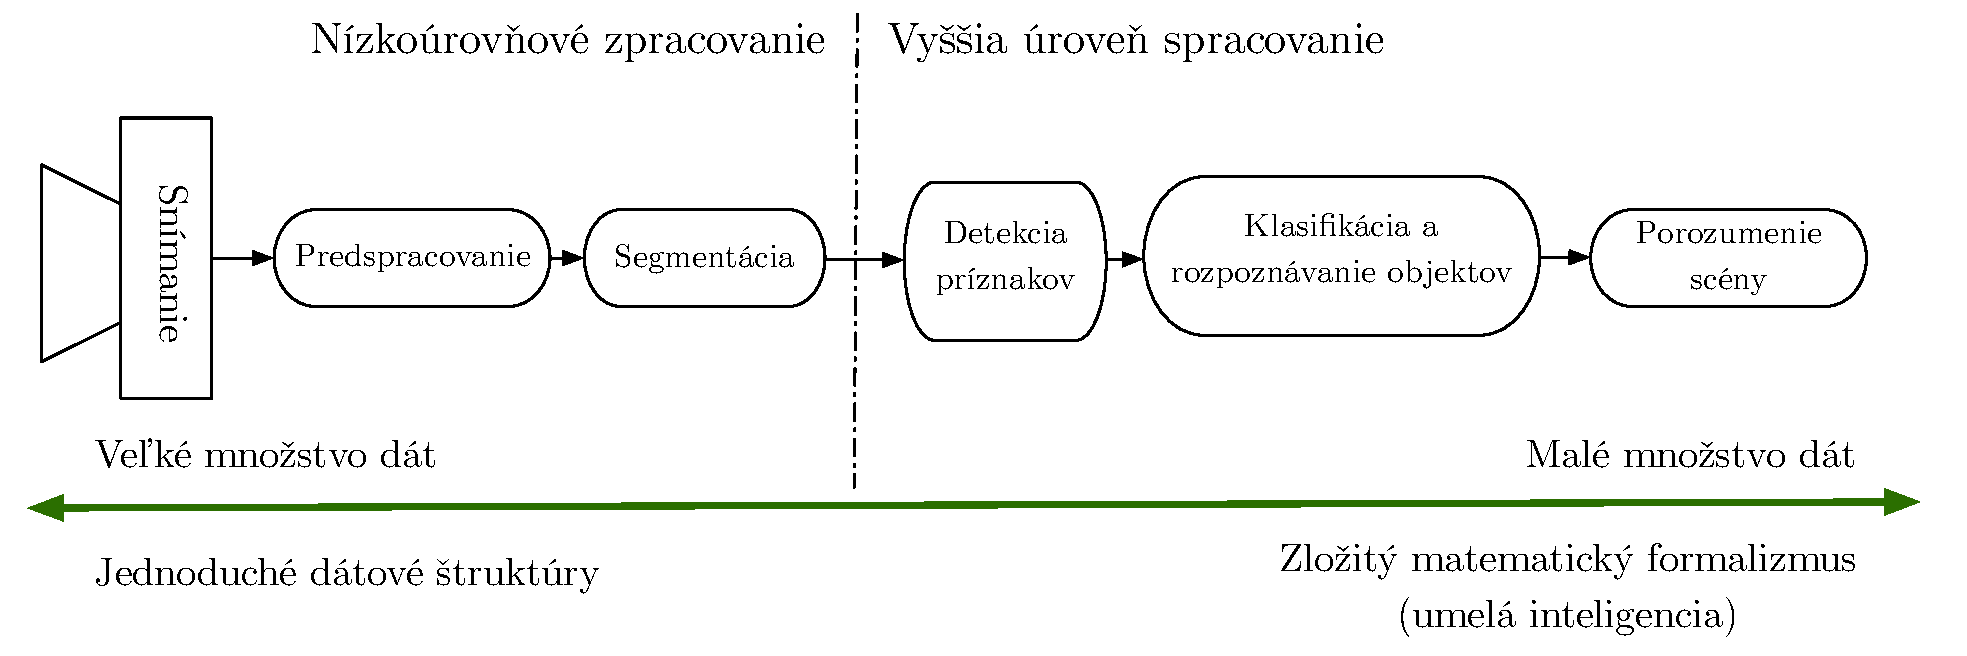
\includegraphics[scale=0.45]{images/phaseCV}
	\caption{Etapy spracovania obrazu}
	\end{center}
\end{figure}

V nasledujúcom texte si postupne opíšeme každú fázu spracovania. 


\subsection{Snímanie}
Základným obmedzením pri vnímaní okolitého 3D sveta, je skutočnosť, že človek dokáže vnímať okolie len 2D, ktorý predstavuje len zjednodušený model 3D okolia.


\subsubsection{Dierková komora}Tento model kamery možno použiť ako prvú aproximáciu mapovania 3D scény do 2D obrazu. Je to analógia toho, čo vzniká na sietnici ľudského oka. \cite{Pin_hole_camera} Obraz sa premieta do obrazovej roviny vzdialenej od dierky o ohniskovej vzdialenosti $f$. V prípade, že sa zrkadlová rovina presunie pred rovinu projekcie z podobnosti trojuholníkov vyplýva nasledujúci vzťah:



\begin{figure}[H]
    \centering
    \begin{minipage}[b]{0.49\textwidth}
        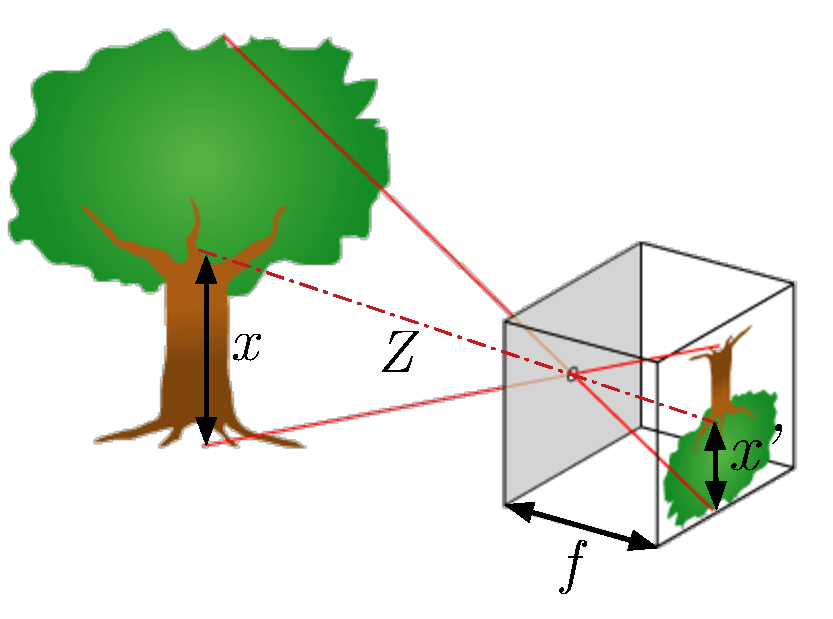
\includegraphics[width=\textwidth]{images/holeCamera}
        \caption{Vyvolanie a prebeh zmeny stavu v komponente}
    \end{minipage}
    \hfill
    \begin{minipage}[b]{0.4\textwidth}
        $$\textit{x}=\frac{X\textit{f}}{Z}$$
        \vspace*{2.5cm}
    \end{minipage}
\end{figure}

Tento výraz predstavuje najjednoduchší model dierkovej kamery, ktorý je základom zložitejších modelov slúžiacich na výpočty napr. pri 3D projekcií. 

\subsubsection{Prevedenie obrazu do počítača (snímanie)}
Je proces transformácie fyzikálneho obrazu do podoby vhodne pre spracovanie za pomoci počítača (matica pixlov) \cite{Analysis_and_Machine_Vision}. Tento proces sa skladá z troch častí: 
\begin{itemize}
\item \textbf{Snímanie} (scaning) - Cieľom prvého kroku je prevod optických veličín na elektrické. Pri použití nekvalitného snímača sa na výstupe objaví veľké množstvo šumu, ktoré len ťažko možno korigovať. Preto je nutné dbať na zaistenie čo najväčšej kvality snímača. 

\item \textbf{Vzorkovanie} - Shanonova veta i vzorkovaní nám vraví, že vzorkovacia frekvencia musí byť aspoň 2x väčšia než je maximálna frekvencia, ktorú obsahuje vzorkovací signál.

$$\textit{f}_{\textit{vzor}} \ge {2} \textit{f}_{\textit{max}}$$

V obrazovej terminológii nám táto veta vraví, že interval vzorkovania musí byť menší alebo rovný polovici rozmerov najmenších detailov na obraze. 

\item \textbf{Kvantovanie} 
Kvantovanie je prevod hodnoty obrazovej funkcie do číselnej hodnoty. Vždy je to proces stratový a nevratný. Počet kvantovacích bodov musí byť dostatočne jemný. Najčastejšie sa v praxi používa 256 úrovní jasu, čo vieme zakódovať do 8 bitov. Výnimku tvoria binárne obrazy, ktoré si vystačia len s dvoma úrovňami 0 a 1. Často sa používa na vytvorenie masky v ktorej možno ľahko nájsť kontúry. Najväčší problém kvantovania na nedostatočný počet úrovní je vnímanie falošných hrán. Možno odstrániť nelineárnym kvantovaním, alebo rozostrením obrazu. 


\item \textbf{Dátové štruktúry} - Najčastejšou reprezentáciu celého obrazu je \textbf{matica} hodnôt. Súradnice prvku v matice zodpovedajú súradniciam pixlu na obraze. Jeho hodnota zodpovedá napríklad jasu.  Okrem nej sa však používajú aj iné ako napríklad kódovanie kontúr segmentovaných objektov. Kontúra je uzavretá hranica objektu, ktorá môže reprezentovať objekt reálneho sveta na obraze a môže byť zdrojom informácii o ňom (tvar, farba, veľkosť) \cite{Analysis_and_Machine_Vision} .

Ďalšou možnosťou kódovania je \textbf{Run-length coding} forma reťazového kódu, použitá hlavne v binárnych obrazoch. 

\textbf{Freemanov (reťazový) kód}  je určený počiatočným bodom a postupnosťou symbolov zodpovedajúcich úsečkám jednotkovej dĺžky v niekoľkých vopred stanovených orientáciách. 

\textbf{Polygonálna reprezentácia hranice} je reprezentácia, ktorá aproximuje oblasť mnohouholníkom. Každá hranica je jednoznačne určená vrcholmi aproximovaného mnohouholníka.

\textbf{Hierarchické dátové štruktúry} obsahuje okrem originálneho obrazu aj jeho zjednodušené časti. Typicky tieto dátové štruktúry pomáhajú znižovať výpočtovú náročnosť a to tak, že sa algoritmus najprv pustí na hrubšiu aproximáciu obrazu, kde sa vytipujú záujmové oblasti a ďalej sa algoritmus aplikuje už len na vybrané časti originálneho obrazu. Základné hierarchické reprezentácie sú pyramídy a kvadrantové stromy \cite{počítačové_videnie_v_praxi}. 

\end{itemize}



\subsection{Predspracovanie obrazu}
Vstupom aj výstupom je obraz na nízkej úrovni abstrakcie. Slúži na zlepšenie obrazu z hadiska ďalšieho spracovania. Môže potlačiť alebo naopak zvýrazniť isté informácie v obraze.\cite{pocitacove_videnie_v_praxi} Metódy spracovania delíme na: 
\begin{itemize}
\item Bodové jasové transformácie
\item Geometrické transformácie
\item Lokálne predspracovanie (filtrácia, ostrenie a detekcia hrán)
\item Obnovenie obrazu pri známej degradácii 
\item Matematická morfológia 
\end{itemize}

\subsubsection{Bodové jasové transformácie}

\textit{Jasová korekcia} - Používa sa pri nerovnomernom osvetlení obrazu. Pokiaľ je porucha
osvetlenia systematická, vieme korigovať odchýlku každého bodu od ideálnej charakteristiky.

\textit{Modifikácia jasovej stupnice} - Na rozdiel od jasovej korekcie, modifikácia stupnice nezávisí na polohe bodu v obraze. Táto modifikácia $T$ prevedie vstupnú jasovú hodnotu na výstupnú a to pomocou známej funkcie (tabuľky) \cite{pocitacove_videnie_v_praxi}. 


\subsubsection{Geometrické transformácie}
Geometrická transformácia 2D obrazu je vektorová transformácia $T$, ktorá zobrazí bod ($x$,$y$) do bodu ($x_0$, $y_0$).  Jedná sa teda o transformáciu súradníc bodov obrazu. Vďaka tomu môžeme odstrániť geometrické skreslenie vzniknuté pri snímaní obrazu (napr. korekcie geometrických porúch objektívu kamery, oprava skreslenia družicového snímku spôsobená zakrivením zemegule).  Z toho vyplýva, že pomocou referenčnej mriežky vieme vyrovnať geometricky deformovaný obraz. Transformačné rovnice môžu byť známe alebo odvodené na základe vstupného a transformačného  obrazu. Pred začiatkom transformácie sa musia nájsť dvojice zodpovedajúcich si bodov (vlícovacie body), ktoré sa na obrázkoch ľahko hľadajú napr. priesečníky vláknitých štruktúr, rohy objektov a pod. Následne sa vykoná transformácia súradníc bodov do nových pozícii. A nakoniec sa musí vykonať aproximácia jasovej funkcie  \cite{Algorithms_and_Applications}.

\begin{figure}[H]
\begin{center}
	
\includegraphics[scale=0.4]{images/transform}
	\caption{Príklad geometrickej transformácie}
	\end{center}
\end{figure}

\subsubsection{Lokálne predspracovanie - filtrácia}
Používa sa na odstránenie vysokofrekvenčných zložiek, čo predstavujú hrany a šum. Pri tejto operácii dochádza k stratení detailov obrazu (rozmazanie)  \cite{Detekcia_a_rozpoznavanie_objektov}.

\textit{Spriemerovanie} - Ide o najjednoduchší prostriedok pre vyhladenie šumu v obraze. Pre každý bod obrazu sa jeho jas nahradí aritmetickým priemerom jasov jeho susedov. Filtrácia spriemerovaním je vlastne špeciálny prípad konvolúcie, kde konvolučná maska vyzerá nasledovne \cite{Detekcia_a_rozpoznavanie_objektov}:

$$\textit{h}=\frac{1}{9}\begin{bmatrix} 1 & 1 & 1 \\ 1 & 1 & 1 \\ 1 & 1 & 1  \end{bmatrix}$$

\textit{Filtrovanie pomocou Gaussovej masky} - Gaussovú masku dostaneme posilnením stredového bodu, prípadne jeho štyroch susedov, tak aby lepšie aproximoval šum s Gaussovým rozdelením \cite{Detekcia_a_rozpoznavanie_objektov}.


\begin{figure}[H]
    \centering
    \begin{minipage}[b]{0.49\textwidth}
        $$\textit{h}=\frac{1}{10}\begin{bmatrix} 1 & 1 & 1 \\ 1 & 2 & 1 \\ 1 & 1 & 1  \end{bmatrix}$$
    \end{minipage}
    \hfill
    \begin{minipage}[b]{0.49\textwidth}
        $$\textit{h}=\frac{1}{16}\begin{bmatrix} 1 & 2 & 1 \\ 2 & 4 & 2 \\ 1 & 2 & 1  \end{bmatrix}$$
    \end{minipage}
\end{figure}


\textit{Mediánový filter} - Medián alebo prostredná hodnota je hodnota, ktorá rozdeľuje postupnosť podľa veľkosti zoradených výsledkov na dve rovnako početné polovice. V štatistike patrí medzi stredné hodnoty. Usporiadame jasové úrovne z lokálneho okolia a vyberieme strednú hodnotu usporiadania. To zabráni, aby krajné extrémy ovplyvnili vybranú hodnotu. Filtrácia však nieje vhodná v obraze, kde sa nachádzajú tenké čiary a ostré rohy \cite{Detekcia_a_rozpoznavanie_objektov}. 


\subsubsection{Lokálne predspracovanie - Detekcia hrán}
Opak filtrácie, zvyšuje vysokofrekvenčné časti spektra (hrán) a odstránenie nízkofrekvenčných častí. Sprievodný javom je aj zvýraznenie šumu v obraze.  Hrana je vektorová veličina, určená veľkostnou a smerom. Pri hranovej detekcii sa využíva vlastnosť gradientu,ktorá hovorí, že hodnota gradientu funkcie dvoch premenných je v oblasti hrany najväčšia. 

\textit{Laplacov operátor} - Tento operátor aproximuje druhú deriváciu a predstavuje rýchlosť zmeny hodnôt jasu. Prejaví sa najmä na strmých alebo izolovaných hranách alebo ju možno použiť na detekciu izolovaných bodov. Bude zvýrazňovať aj šum \cite{Detekcia_a_rozpoznavanie_objektov}.

\begin{figure}[H]
    \centering
    \begin{minipage}[b]{0.49\textwidth}
        $$\textit{h}_1=\begin{bmatrix} 0 & 1 & 0 \\ 1 & -4 & 1 \\ 0 & 1 & 0  \end{bmatrix}$$
    \end{minipage}
    \hfill
    \begin{minipage}[b]{0.49\textwidth}
        $$\textit{h}=\begin{bmatrix} 0 & 0 & -1 & 0 & 0 \\ 0 & -1 & -2 & -1 & 0 \\ -1 & -2 & 16 & -2 & -1 \\ 0 & -1 & -2 & -1 & 0 \\ 0 & 0 & -1 & 0 & 0  \end{bmatrix}$$
    \end{minipage}
\end{figure}


\textit{Sobelov operátor} - Aproximuje prvé parciálne derivácie. Nakoľko samotná derivácia zvýrazňuje šum, vykonáva ja vyhladzovanie. Pre každý smer hrán existuje špeciálna maska \cite{Detekcia_a_rozpoznavanie_objektov}.

\begin{figure}[H]
    \centering
    \begin{minipage}[b]{0.49\textwidth}
        $$\textit{h}_1=\begin{bmatrix} 1 & 2 & 1 \\ 0 & 0 & 0 \\ -1 & -2 & -1  \end{bmatrix}$$
    \end{minipage}
    \hfill
    \begin{minipage}[b]{0.49\textwidth}
        $$\textit{h}_2=\begin{bmatrix} 0 & 1 & 2 \\ -1 & 0 & 1 \\ -2 & -1 & 0  \end{bmatrix}$$
    \end{minipage}
\end{figure}


\begin{figure}[H]
\begin{center}
	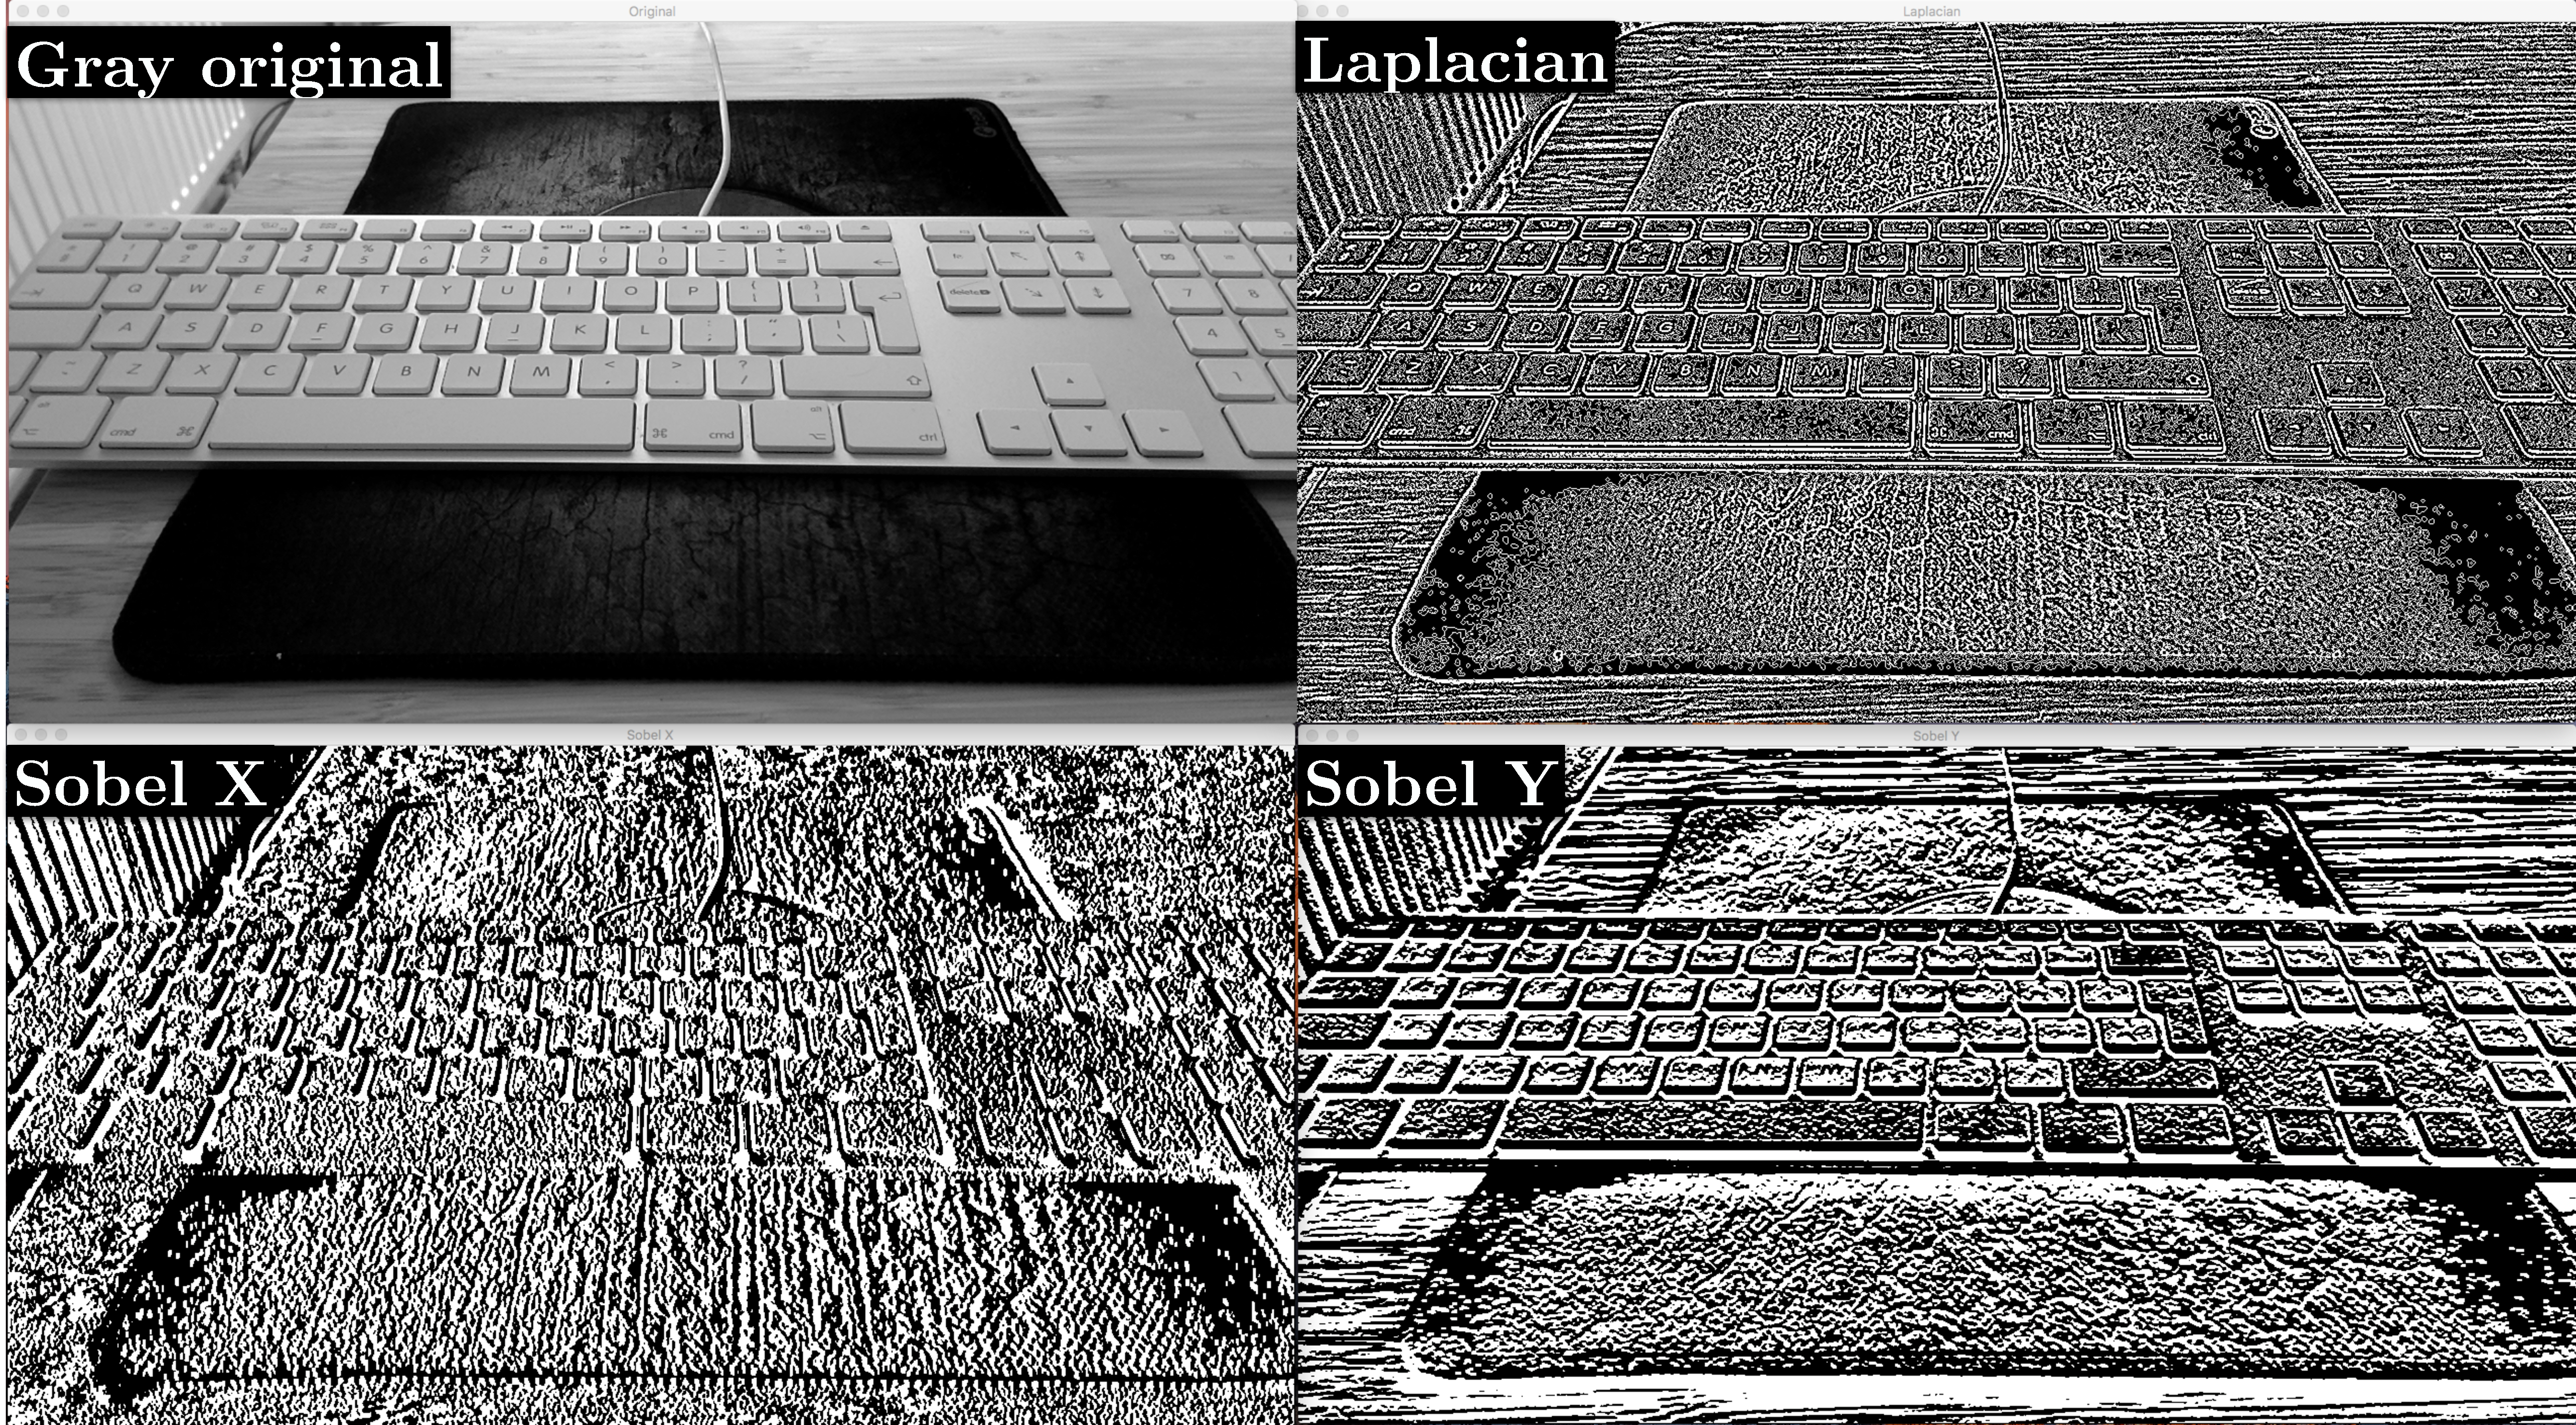
\includegraphics[scale=0.16]{images/edgeDetector}
	\caption{Vzájomné porovnanie algoritmou pre detekciu hrán}
	\end{center}
\end{figure}


\subsection{Segmentácia obrazu}
Segmentácia je rozdelenie obrázku na časti, ktoré silne korelujú s objektami reálneho sveta. Pri čiastočnej segmentácii je cieľom rozdeliť obraz na časti, ktoré sú homogénne z hľadiska vybranej vlastnosti (farba, jas, odrazivosť atď …) Cieľom segmentácií v počítačovom videní je značná redukcia objemu dát. Nejednoznačnosť obrazových dát je hlavným problémom segmentačného procesu. \cite{pocitacove_videnie_v_praxi} Segmentačné metódy možno rozdeliť na tri skupiny: 


\begin{itemize}
\item Prahovanie
\item Segmentácia založená na hranách (diskontinuita)
\item Segmentácia založená na oblastiach (podobnosť)
\end{itemize}

\subsubsection{Prahovanie}
Najjednoduchšia segmentačná technika. Je založená na predpoklade, že jednotlivé objekty majú konštantnú obrazivosť, či pohltivosť svetla na svojom povrchu. Je to transformácia, ktorá zobrazuje vstupný obraz $f(i, j)$ na výstupný obraz $g(i, j)$ nasledovne \cite{fit_trasholding} : 
$$g (i{,}j)=1 {,}\quad {ak} f(i{,}j)\ge T$$
$$g (i{,}j)=0 {,}\quad {ak} f(i{,}j)  < T$$


Z toho vyplýva, že na segmentovanie objektov od pozadia sa používa jasová konštanta, ktorá sa nazýva prah. 


\textit{Globálne prahovanie} - Je to technika. ktorá je vhodná, keď sa objekty na scéne diametrálne líšia svojimi charakteristikami. V takom prípade môžeme nastaviť prah ako interval platných hodnôt. Príklad použitia môžeme vidieť na obrázku s kačkou. Originálny obrázok sa konvertuje do HSV farebného priestoru, ktorý umožňuje lepšiu prácu s odtieňmi farieb spôsobené nehomogénnym osvetlením. Následne sa aplikuje filter ktorý prepustí len hodnoty v danom intervale \cite{fit_trasholding}.

\begin{figure}[H]
\begin{center}
	
\includegraphics[scale=0.25]{images/trasholding_duck}
	\caption{Detekcia tela kačky na základe prahovania}
	\end{center}
\end{figure}


\textit{Lokálne prahovanie} - Málokedy je možné použiť jednu hodnotu prahu (alebo interval) na celý obraz, z dôvodu fyzikálnym podobnostiam objektov v scéne a  nehomogénnemu osvetleniu scény. Preto sa často používajú metódy lokálneho prahovania. Algoritmy sa počítajú v malých regiónoch obrazu. Tak dostaneme rôzne prahové hodnoty pre rôzne regióny rovnakého obrazu a to nám dáva lepšie výsledky u snímok s rôznym osvetlením \cite{fit_trasholding}\cite{openCV_trasholding}. Môžeme ho definovať takto : 
$$T=T(f {,} f_c){,}$$

kde $f_c$ je časť obrazu v ktorej sa určuje prah. 

\begin{figure}[H]
\begin{center}
	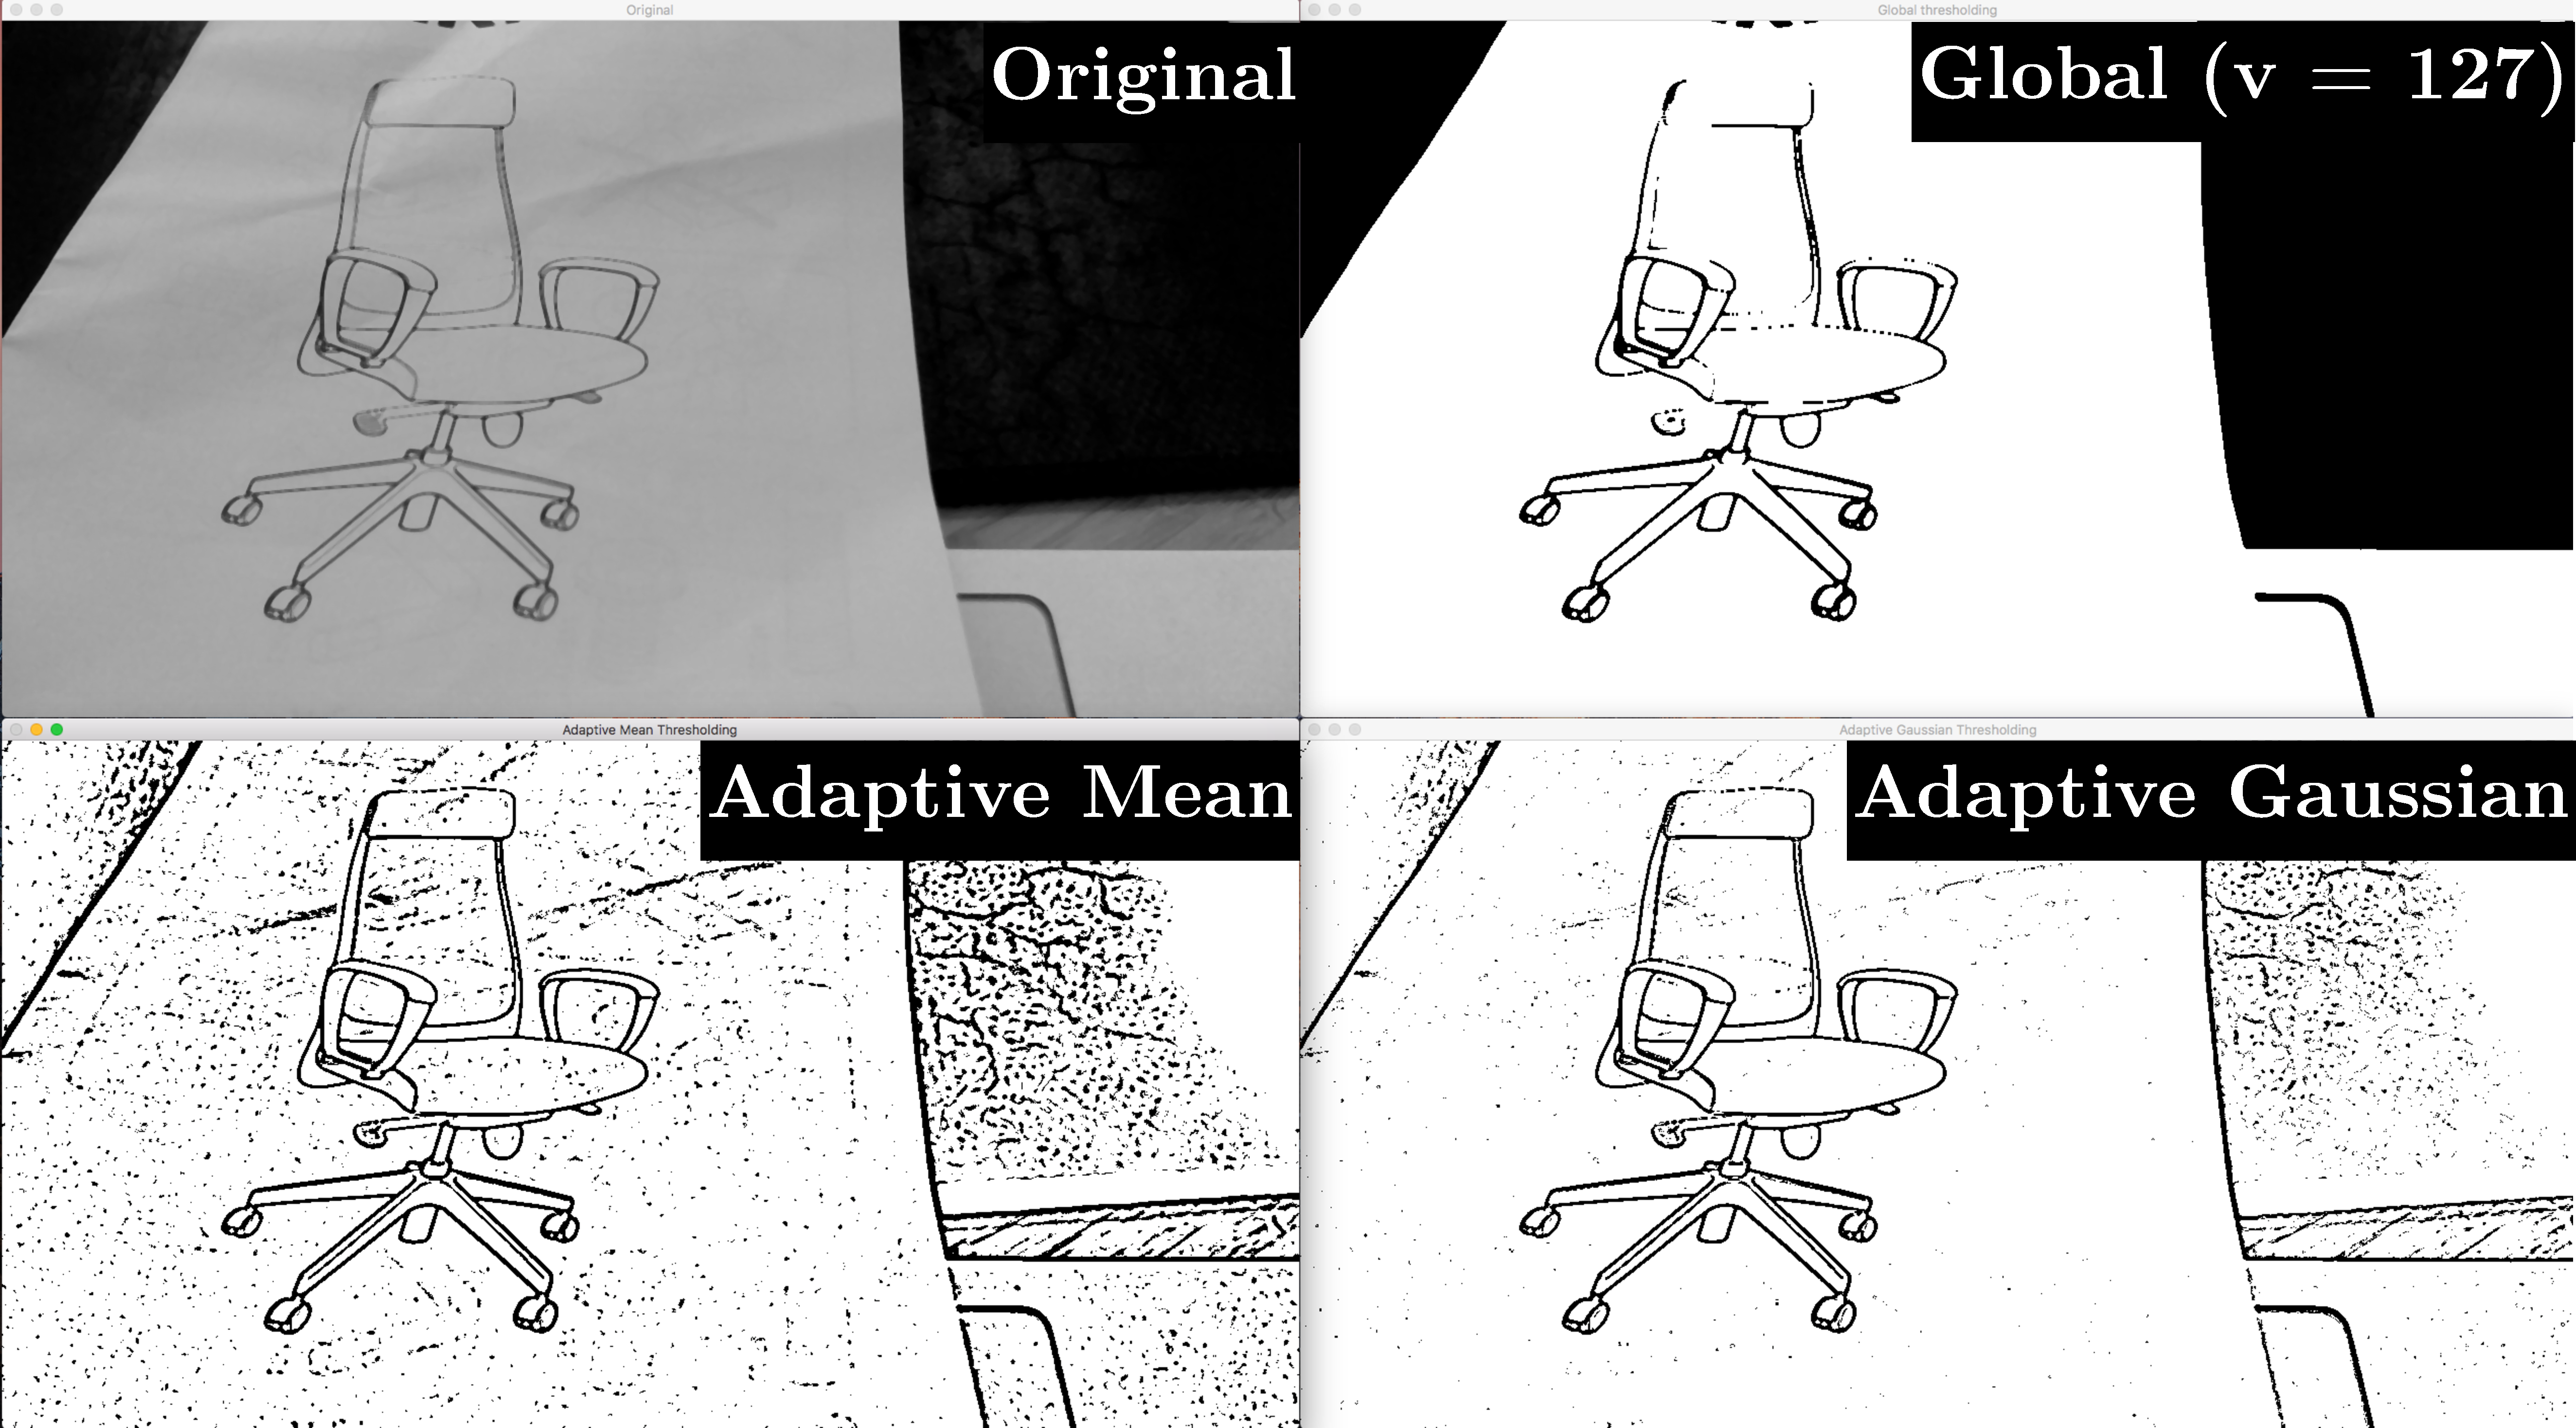
\includegraphics[scale=0.15]{images/trasholding}
	\caption{Porovnanie výsledkov metod lokalneho prahovania}
	\end{center}
\end{figure}



\subsubsection{Segmentácia na základe detekcie hrán}
Techniky založené na informáciach, ktoré poskytujú hrany v obraze. Preto je  nutné si vysvetliť aký rozdiel je medzi pojmom hrana a hranica. Hrana je miesto kde sa skokovito mení hodnota obrazovej funkcie. Pre účely segmentácie sú však dôležitejšie hranice regiónov.  Región je množina súvislých bodov a hranicu regiónu je množinu bodov, ktoré sú súčasťou regiónu, ale zároveň aspoň jeden z ich susedov nepatri regiónu. Takáto hranica tvorí vnútornú hranicu regiónu \cite{pocitacove_videnie_v_praxi}. 

\textbf{Metóda sledovania hranice}
Táto metóda pracuje na binárnom obraze. Vnútornú hranicu získame tak, že  prehľadávame obraz zľava doprava, zhora dole, pokiaľ nenarazíme na bod patriaci regiónu. Tento bod pridáme do hranice. Nasledovne prehľadávame okolie tohoto bodu v protismere hodinových ručičiek od posledne navštíveného bodu. Pokiaľ narazíme na bod, ktorý je patriaci do rovnakého regiónu, pridáme ho do hranice. Tento postup opakujeme dokiaľ sa nedostaneme naspäť k počiatočnému bodu \cite{pocitacove_videnie_v_praxi}. 

Algoritmus nájde iba vnútorne hranice. Pokiaľ chcem nájsť vonkajšie hranice, môžeme ich získať tak že, nájdeme vnútorné. Potom vonkajšiu hranicu tvoria body, ktoré sme pri vyhľadávaní vnútornej hranice testovali, ale nepatrili do regiónu. 

Tento algoritmus funguje pre oblasti väčšie než 1 pixel.  Ide o veľmi obľúbený a účinný algoritmus, ktorý sa veľmi často používa.

\textbf{Cannyho detektor} - jeden z najlepších a najpoužívanejších algoritmov pre detekciu hrán, ktorý je založený na hľadaní hodnoty gradientu a spoľahlivosti bodu na základe susedných bodoch. Požiadavky na úspešnosť sú presnosť, minimálny počet chýb a jednoznačnosť. 

Prvý krok algoritmu je eliminácia šumu použitím \textit{Gaussovho filtra}.  Následne nájdeme miesto a smer gradientu použitím \textit{Sobelového operátora}. Ďalej musíme odobrať z hodnôt gradientu  body, ktoré nie sú lokálne maximá. Napríklad, ak máme pixel, ktorým prechádza zvislá hrana, musí byť jeho ľavý a pravý sused nižšej hodnoty, aby bol uznaný  ako skutočná hrana. V poslednom kroku musíme uplatniť metódu \textit{prahovania s hysteréziou}. Zvolíme si minimálny (T1) a maximálny (T2) prah medzi ktorým môže gradient kolísať.  Ak je hodnota gradientu pixlu vyššia než T2 je pixel označený ako hranový. Ak hodnota bodu leží medzi T1 a T2 bod je uznaný ako hranový len vtedy, ak leží vedľa suseda označeného ako hranový \cite{cannyho_detektor}.


\textbf{Hľadanie hraníc Houghovou transformáciou} - pomocou tejto metódy je možné nájsť v obraze objekt, ktorého tvar je možné popísať analytickým výrazom (priamka, kruh, elipsa a iné). Veľkou výhodou je invariantnosť metódy na zmenu mierky, pootočenie a veľká odolnosť voči pôsobeniu šumu v obraze \cite{houghova_transformacia}. 

\subsubsection{Segmentácia založená na spájaní a delení oblastí}
Metódy tejto kategórie nehľadajú hranice jednotlivých regiónov ale snažia sa o nájdenie oblastí priamo. Hlavná myšlienka je založená na klasifikácii obrazu do niekoľkých spojitých homogénnych podoblastí, ktoré sú vzájomne disjunktné, pričom zjednotením podoblastí je celý obraz \cite{pocitacove_videnie_v_praxi}.
$$R=\bigcup_{i=1}^s R_i{,}\quad R_i\bigcap R_j=0{,}\quad{pre}\quad i\neq j$$

Medzi základné podmienky segmentácie patrí kritérium homogenity:
$$H(R_i)={THRUE}{,}\quad \textit{i}=1{,}2{,}{...}{,}s{,}$$
$$H(R_i \cup R_j)={FALSE}{,}\quad \textit{i} \neq \textit{j}{,}\quad R_i { \ je \ susedné \ k \ } R_j $$

kde S je celkový počet regiónov v obraze a $H(R_i)$ je hodnota binárne homogenity regiónu $R_i$. Prvá podmienka sa týka vlastností, ktoré musia spĺňať pixle v segmentovanom regióne, druhá určuje, že susedné regióny $R_i$ a $R_j$ majú odlišné veľkosti. Existuje veľké množstvo metód založených na segmentácii regiónov, pričom sa z výkonnostného hľadiska veľmi nelíšia. Veľkou výhodou metód tejto kategórie je odolnosť voči šumu, preto v prípadoch veľkého zašumenia obrazu sú lepšou cestou oproti metódam založených na detekcii hrán avšak na úkor väčšej výpočtovej náročnosti.  

\subsection{Príznaky a rozpoznávanie}
Proces segmentácie zaručuje, že obraz bol rozdelený do vzájomne disjunktných častí. To však vo väčšine prípadov nestačí a je nutné rozdeliť jednotlivé regióny tak, aby korelovali s objektami reálneho sveta. To si však vyžaduje vytvoriť exaktný popis oblastí. Až na základe neho môže klasifikátor rozdeliť jednotlivé objekty do tried.  Z toho vyplýva, že proces segmentácie bezprostredne predchádza procesu klasifikácie.  Tento proces však nieje vždy nutný. Ak je cieľom odlíšenie objektov od pozadia výsledkom takejto snahy je binárny obraz, kde objekty záujmu sú biele a nepodstatné okolie čierne \cite{Analysis_and_Machine_Vision}.
Rozpoznávanie je klasifikačná úloha. Existujú dve základné formy opisu objektu, podľa nich delíme aj metódy rozpoznávania na dve základné skupiny: 

\begin{itemize}
\item Príznakové - príznaky popisujúce objekt 
\item Syntaktické - pomocou primitív (formálne gramatiky, produkčné pravidlá, fuzzy logika)
\end{itemize}

\subsubsection{Skalárne deskriptory}
Je to výsledok merania ktorý kvantifikuje nejakú vlastnosť. Medzi jednoduché skalárne deskriptory  patria napríklad veľkosť,  okrúhlosť, obvod dĺžka hlavnej osi, uhol hlavnej osi, ťažisko,  projekcia, výška, šírka, výstrednosť, pozdĺžnosť, pravouhlosť, smer, nekompaktnosť, Feretov priemer a iné. 

Tvarové invarianty. Sú to deskriptory tvaru objektu, ktoré sú invariantné k určitej triede transformácii.
Často používané sú aj viacrozmerné skalárne deskriptory medzi ktoré patrí napríklad obraz, histogram alebo kombinácia skalárnych deskriptorov  \cite{Analysis_and_Machine_Vision}. 

\subsubsection{Momenty}

Jeho všeobecná definícia je takáto:
$$m_{pq}=\sum_{i=\infty}^\infty \sum_{i=\infty}^\infty i^p j^q f(j,j)$$
Na základe momentov je možné vypočítať charakteristiky oblastí, ako napríklad ťažisko takto: 
$$x_c=\frac{m_{10}}{m_{00}}\ {,}\quad y_c=\frac{m_{01}}{m_{00}}$$
Následne je možné definovať centrálny moment, ktorý je invariantný voči posunu. 


\subsubsection{Štatistické metódy rozoznávania}
Tieto metódy úzko súvisia s pojmom klasifikácia a ich základom sú štatistické postupy. Klasifikátor je nástroj, ktorý na základe príznakov zaradí objekty do tried. Funkcie, ktoré oddeľujú jednotlivé triedy sú diskriminačné funkcie \cite{pocitacove_videnie_v_praxi}. Pokiaľ ich vieme znázorniť ako priamku, ide o lineárne klasifikároty. Existujú tri typy klasifikátorov: 

\begin{itemize}
\item Deterministický  – Založený na diskriminačných funkciách, určitá vzorka je vždy zaradená do určitej triedy 
\item Stochastický -  Založený na pravdepodobnosti, že klasifikátor zaradí niektorý z objektov do nesprávnej triedy (každé rozhodnutie nesie riziko chyby).  Napríklad Bazesov klasifikátor
\item Heuristický - neurónové siete, k-najbližších susedov, logistická regresia, Support Vector 
Machines (SVM), rozhodovacie stromy (Decision trees) 
\end{itemize}

\subsection{3D snímanie priestoru}
Základným princípom je projekcia lúčov odrazených od 3D objektov sveta na 2D plochu snímača.  \cite{Analysis_and_Machine_Vision} Pri tomto procese však dochádza k rôznym efektom pri ktorých sa stráca veľa informácii. Napríklad premietanie viacerých bodov 3D scény do jedného bodu na 2D senzore, prekrývanie objektov alebo aj šum. Existujú však metódy, ktorým sa darí dané problémy eliminovať a dosiahnuť tak  hlavný cieľ, ktorým je porozumieť 3D snímanej scéne. Metódy 3D snímania možno deliť do dvoch základných skupín: 

\begin{itemize}
\item Pasívne metódy
\item Aktívne metódy 
\end{itemize}

\subsubsection{Pasívne metódy - stereo videnie}
Tieto metódy potrebujú pre snímanie scény zisk z dvoch kamier zo vzájomne rôznou pozíciou a ľubovolným uhlom. 

\begin{figure}[H]
\begin{center}
	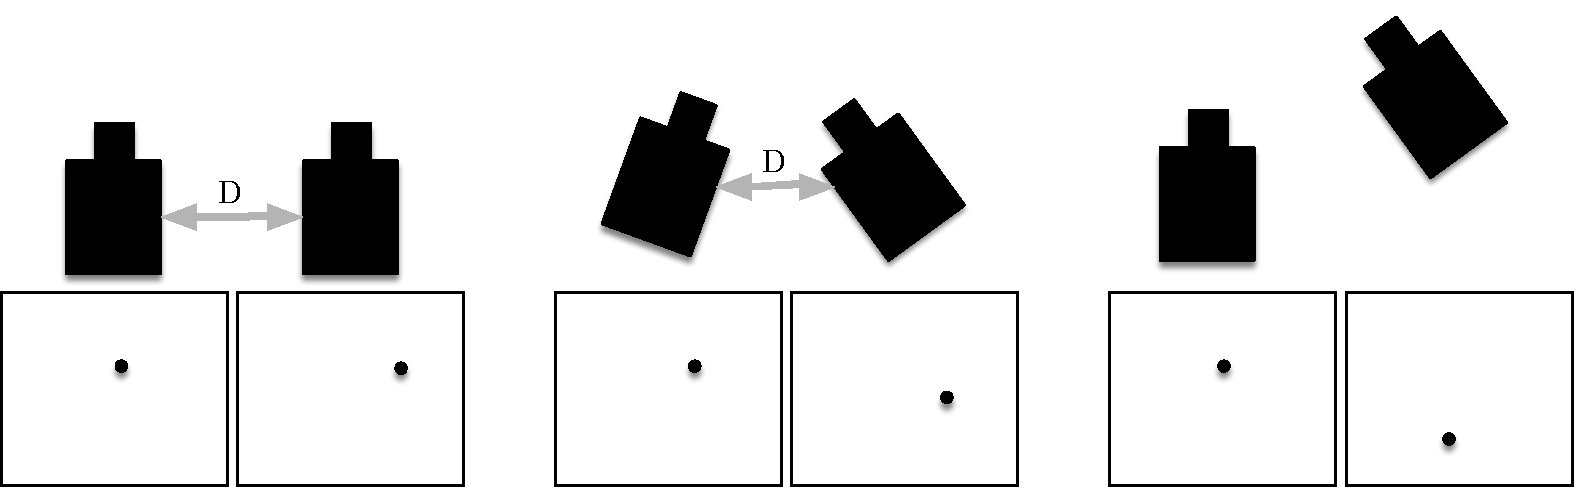
\includegraphics[scale=0.5]{images/3D_cameraPos}
	\caption{Možnosti vzájomných polôch dvoch kamier}
	\end{center}
\end{figure}


V nasledujúcom texte sa však obmedzíme na situáciu A. Obe kamery snímajú scénu bod rovnakým uhlom a zo známou vzdialenostnou medi nimi. Táto situácia je rovnaká ako v ľudskom videní, len namiesto očí pracujeme s kamerami. Táto metóda je založená na triangulácii, čo je orientácia snímkovej dvojice \cite{Algorithms_and_Applications}. 

\begin{figure}[H]
\begin{center}
	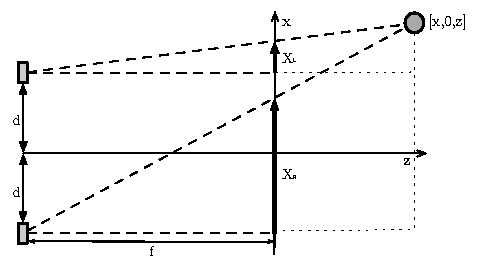
\includegraphics[scale=1.8]{images/stereoscope}
	\caption{Výpočet vzdialenosti na základe tirangulácie}
	\end{center}
\end{figure}

podobnosti trojuholníkov potom platí:


\begin{figure}[H]
    \centering
    \begin{minipage}[b]{0.49\textwidth}
        $$\frac{X_L}{f}=\frac{x-d}{z}\ {;}\quad \frac{X_R}{f}\frac{x+d}{z}$$ 
    \end{minipage}
    \hfill
    \begin{minipage}[b]{0.49\textwidth}
       $$ z=\frac{-2df}{X_L-X_R}$$
    \end{minipage}
\end{figure}



Z obrázka vyplýva, že pri známych veličinách $f$ (ohnisková vzdialenosť) a $d$ (vzdialenosť kamier od seba) vieme vypočítať pre každý pixel jeho hĺbku. Je to možné na základe disparity, čo je rozdiel medzi polohou bodu snímaného jednou kamerou oproti pozícii toho istého bodu snímaného druhov kamerou. Takže každý pixel scény pozorovanej dvoma kamerami má istú hodnotu disparity. Čim je vzdialenosť od kamier väčšia, tým je táto hodnota menšia a čím je vzdialenosť menšia hodnota disparity je väčšia. Implementácia je veľmi náročná. Vyžaduje si presné technické špecifikácie kamier a algoritmy, ktoré dokážu nájsť korešpondujúce body sú zložité. Najpoužívanejším je RANSAC \cite{pocitacove_videnie_v_praxi}. 

Pre kamery ktoré nie sú umiestnené v rektifikovanej  polohe sa používa epipolárna geometria. 


\subsubsection{Postupné ostrenie obrazu }
Pokiaľ máme k dispozícii kvalitnú kameru, ktorá dokáže selektívne zaostrovať na určitú vzdialenosť, vieme postupným procesom získať hĺbku každého pixlu, podľa momentu, kedy bol správne zaostrený. To, či je obraz na určitom mieste zaostrený, je možné určiť pomocou rôznych lokálnych operátorov známych z detektorov hrán (kapitola xxx). 


\subsubsection{Aktívna triangulácia }
\label{sec:activeDeep}
Základným znakom je pridanie dodatočnej informácie do scény. Táto informácia môže byť reprezentovaná laserom, ifražiaričom alebo projektorom. Tieto metódy sa charakterizujú ako optické metódy merania vzdialenosti. Optické metódy sú také, ktoré meranie vykonávajú určitým optický lúčom.  Meranie je teda realizované postupným premietaním vzoru na predmet a následným zachytením kamerou. Podľa deformácie premietaného vzoru je možné následne určiť hĺbkovú mapu priestoru.

\subsection{Analýza pohybu }
Väčšina aplikácii, ktoré rieši počítačové videnie spočíva v nájdení, rozpoznaní a následnom sledovaní objektu, ktorý sa pohybuje po scéne. 

Veľmi používaná je detekcia samotného pohybu. V tomto druhu aplikácii statická kamera sleduje určitú scénu a je cieľom zistiť nežiadaný pohyb na sledovanej scéne. Ide o veľmi jednoduché aplikácie implementované napríklad aj v bezpečnostných kamerách ako inteligentná spúšť nahrávania.  Algoritmy nemajú za úlohu riešiť smer ani trajektóriu pohybu, sú schopné len vyrátať o koľko sa zmenila scéna oproti referenčnej vzorke. Jedna z najpoužívanejších metód je diferenčná metóda. Detekcia lokalizácia a predikcia pohybujúceho sa predmetu oproti detekcii samotného pohybu tieto metódy majú  za úlohu zistiť aj trajektóriu a vyrátať predikciu ďalšej polohy objektu. Medzi najkomplikovanejšie situácie patria tie, pri ktorých sa naraz môže pohybovať kamera ja objekt súčasne.

\subsubsection{Kalmanov filter}
Pri analýze pohybu objektu veľmi často dochádza k spájaniu, zatieneniu, či zmiznutiu sledovaného  objektu na obraze. Z toho dôvodu by sme potrebovali prostriedok, ktorý by spĺňal nasledovné podmienky: 


Očakávaná hodnota odhadu by mala byť rovná očakávanej hodnote stavu - Potrebujeme priemernú hodnotu odhadovaného stavu. Je nežiaduce aby odhadovaná hodnota bola posunutá nahor alebo nadol. 
Chceme nájsť taký prostriedok pre odhad, ktorý má čo najmenšiu variáciu chyby - odhadovaná a následne nameraná hodnota by sa mala líšiť minimálne. 



Všetky tieto predpoklady spĺňa práve Kalmanov filter, avšak je možné ho použiť len vtedy, ak  meraný systém je opísateľný iným lineárnym systémom. Je to z dôvodu aby Kalmanov filter nebol ovplyvnený šumom. Kalmanov filter teda hľadá najoptimálnejším odhad budúceho stavu na základe stavov minulých a popisu systému.  Existuje už vyše 50 rokov, no stále je jedným z najdôležitejším, a najodporučanejším algoritmom \cite{Kalman_web}.

\begin{figure}[H]
\begin{center}
	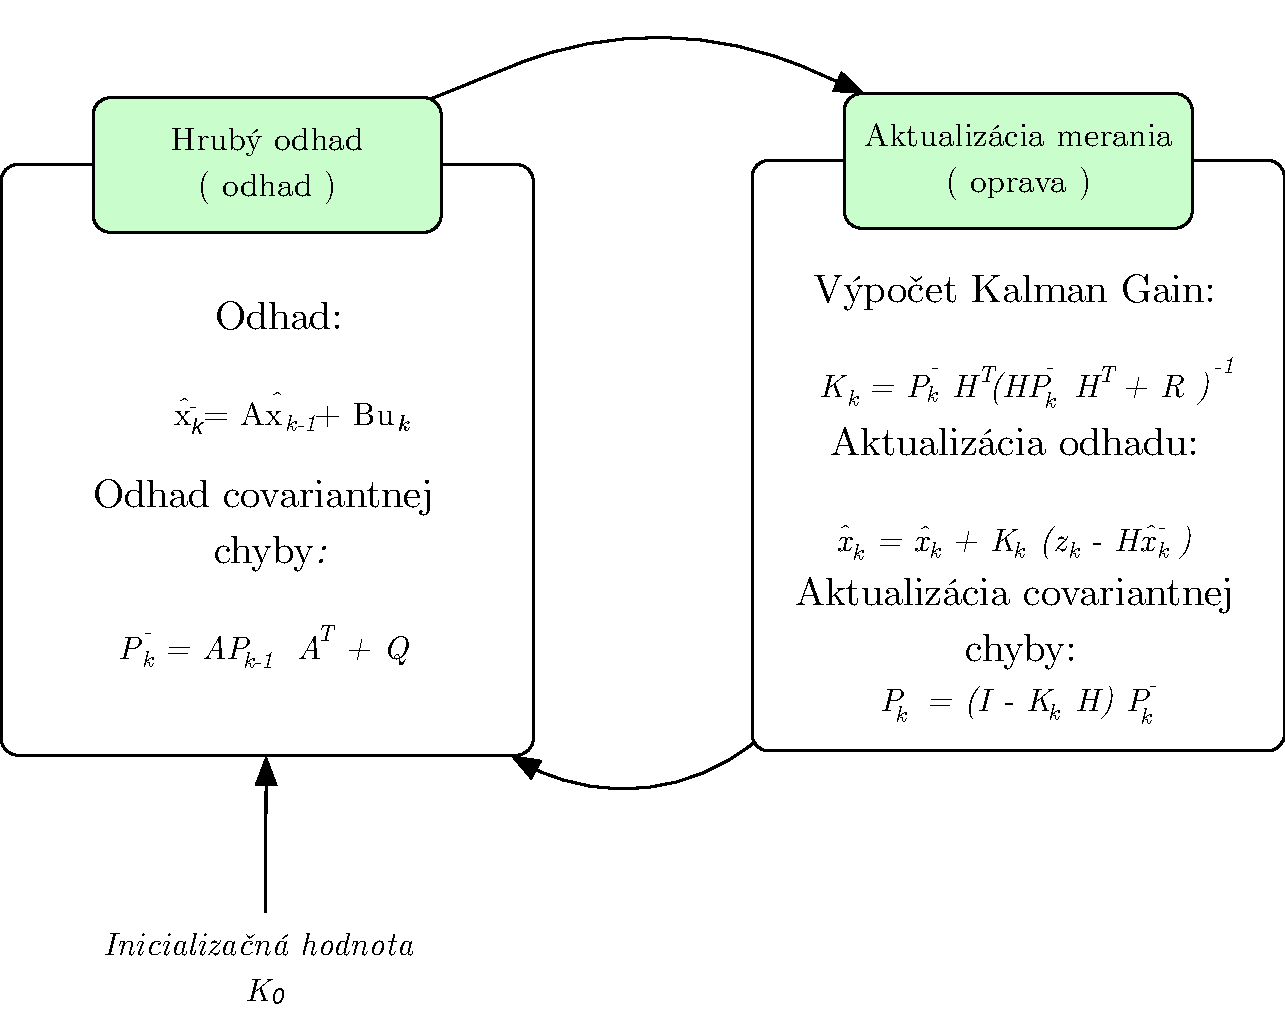
\includegraphics[scale=0.33]{images/kalman}
	\caption{Popis algoritmu Klmanového filtra}
	\end{center}
\end{figure}

Hrubý odhad je predchádzajúci odhad polohy pred aktualizáciou merania. V časti aktualizácia merania už naozaj odhadneme nasledujúci krok. Z rovnice Kalman Gain alebo výpočet kalmanového zisku vyplýva, že ak je šum z merania R veľké, nebudeme dávať veľkú váhu meraniu pri výpočte ďalšieho kroku. Naopak ak je šum merania R malé, priradíme meranej hodnote veľkú váhu pri ďalšom kroku.   % viz. obsah.tex / see obsah.tex
  \chapter{Návrh riešenia problému}
\section{Existujúce problémy}
Pred zahájením tvorby aplikácie je nutné oboznámiť sa s problémami, ktoré je nutné aby aplikácia riešila. Na prvý pohľad  sa môže zdať, že  počítanie ľudí je jednoduchý proces. Predpokladajme, že virtuálna brána je umiestnená pri vstupe do miestnosti. Proces prechodu osoby znamená zvýšenie počítadla prechodov osôb a na základe smeru danej osoby dekrementovať alebo inkrementovať počet osob nachádzajúcich sa v miestnosti. Systém musí byť navrhnutý tak, aby bol schopný detekovať a sledovať aj viacero ľudí ktorý v jedenom okamihu prechádzajú cez virtuálnu bránu rovnakým alebo odlišným smerom.  Jeden z najväčších problémov je však dynamickosť prostredia, kde by aplikácia mala byť nasadená. Rýchle svetelné zmeny okolia,  nepredvídateľné pohyby ľudí na scéne (môže zastať, dotýkať sa, ťahať / tlačiť iný objekt)  toto všetko je nutné riešiť, tak aby aplikácia dosiahla čo najväčšej presnosti. 

\section{Konceptuálny návrh systému}
Z problémov opísaných v sekcii 3.1 je jasné, že jednoduché systémy typu Infračervená závora, nebudú mať dostatočne veľkú presnosť vzhľadom na prechody viacerých osôb v jednom časovom okamihu. Je nutné oprieť sa o metódy, ktoré vedia zaznamenať viac informácii o objekte, ktorý prechádza vymedzeným priestorom (tvar, rýchlosť, veľkosť, smer, atd …). 

Jedným z najkomplexnejších prostriedkov, ako dostať dáta do počítača na spracovanie je kamera, ktorá nám poslúži ako senzor.  Umiestnime ju na vrchnú priečku prechodu tak, aby snímala osoby z vrchu. Táto pozícia je najlepšia, lebo eliminuje možnosti zatienenia sledovaného objektu iným objektom na scéne.  

\begin{figure}[H]
  \centering
  \begin{minipage}[b]{0.2\textwidth}
    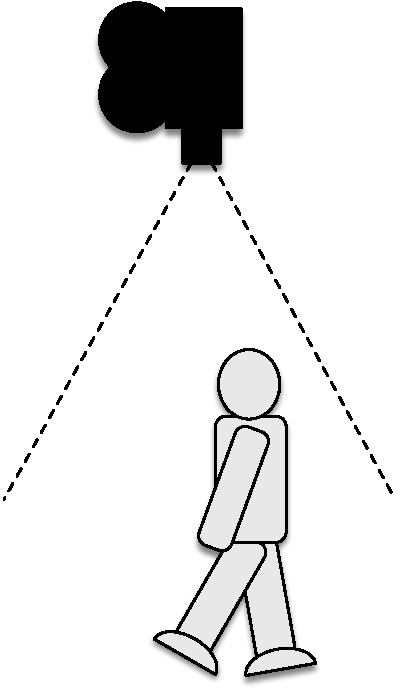
\includegraphics[width=\textwidth]{obrazky/konceptSnimania}
    \caption{Poloha kamery.}
  \end{minipage}
  \hfill
  \begin{minipage}[b]{0.5\textwidth}
    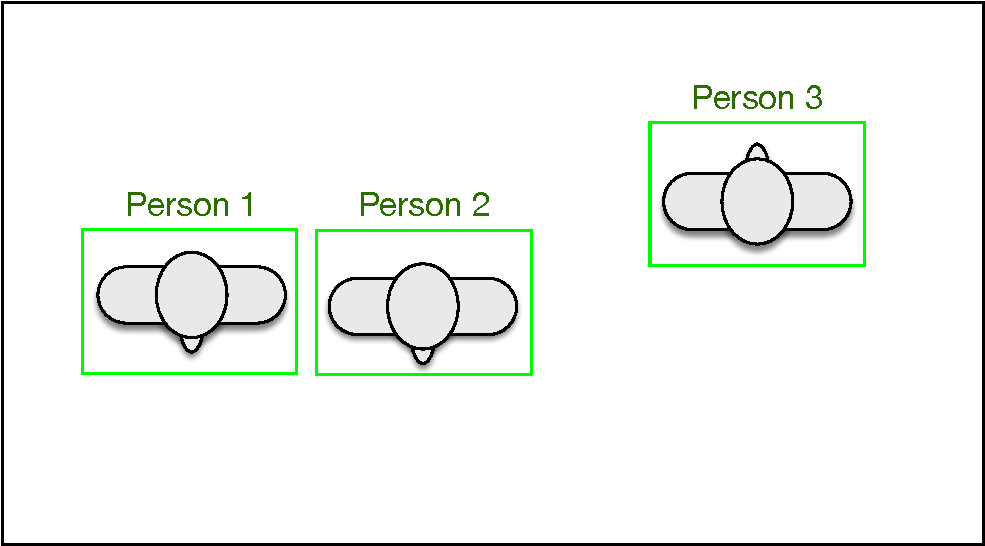
\includegraphics[width=\textwidth]{obrazky/pohladZhora}
    \caption{Obraz snímanej scény}
  \end{minipage}
\end{figure}

\section{Výber snezora (kamery)}
Výber vhodného snímača priestoru virtuálnej brány je veľmi dôležitý. Ak senzor bude snímať dáta, ktoré sú enormne zaťažené šumom, realizácia funkčného algoritmu bude veľmi náročná, v niektorý prípadoch až nemožná. Táto práca sa zameriava na dva typy vhodných kamier \textbf{3D kamery} a\textbf{ 2D  RGB kamery}.

\subsection{3D kamery}
Keďže  koncept snímania priestoru sa opiera o snímanie z výšky, veľmi silným kandidátom sú aktívne 3D kamery. Veľká výhoda je meranie na základe tvorby hĺbkového obrazu(kapitola XXX). Vďaka tomu, má meranie vysokú presnosť, nepotrebuje osvetlenie priestoru ani kontrastné prostredie.  Ďalšou veľkou výhodov je informácia o výške osoby, ktorá prechádza. Táto informácie je použiteľná v mnohých aspektoch ďalšieho spracovania. Na druhej strane technológia aktívneho 3D hĺbkomera je náchylná na priame slnečné lúče. Tie dokážu merania veľmi znehodnotiť. Vo svojej práci som otestoval tri rôzne aktívne hĺbkomery: 

\begin{itemize}
\item Kinect 360
\item Orbbec Astra S
\item Intel RealSence SR300

\end{itemize}

\subsubsection{Testovanie}
Testovanie spočívalo v umiestnení všetkých troch kamier na vhodné miesto, kde sa nahrával záznam po dobu 10 minút. Vďaka tomu je zaručené, že všetky tri kamery boli vystavené rovnakému prostrediu a boli nahrávané za rovnakých svetelných podmienok.  Počas nahrávania bol udržiavaný konštantný pohyb osôb cez bránu. Pre ohodnotenie kvality jednotlivých záznamov bola použitá \textbf{metrika hodnotenia} založená na priemernom počte nenameraných pixelov na jednom snímku. Nenameraný pixel znamená, že sa nachádza nekonečne ďaleko alebo ide o chybu merania spôsobená tvarom objektu (ostrá hrana), slnečným žiarením, materialom oklitého prostredia alebo iné. \textit{Metóda pre výpočet hodnotiacej metriky konverguje k objektívnemu výsledku len vtedy, ak každý objekt scény sa nachádza v zornom poli kamery, ktoré udáva jej výrobca.}  

\subsubsection{Kinect 360}
Kinect sníma frekvenciou 30 Hz. Hĺbka je snímaná s presnosťou na 11 bitov, čiže hĺbka jedného pixela môže nadobudnúť hodnoty od 0 do 2047.  Pracovný rozsah senzora je  1,2 - 3,5 metra.  Využíva technológiu vyvinutú firmou PrimaSence. V ľavej časti senzora sa nachádza IR projektor s vlnovou dĺžkou svetla 830nm. Generátor kóduje informáciu do svetelných vzorov, ktoré sa odrazom od predmetov pred senzorom deformujú. Odraz IR svetla je zachytený senzorom v pravej časti senzora a z veľkosti deformácii je vypočítaná hĺbková mapa. Používa USB 2.0 rozhranie. 

Kedže od spoločnosti Microsoft neexistuje oficialna podpora operačných systémov Unixového typu, na čítanie obrazu z kameri som použil knižnicu vyvíjanú komunitou \textit{libfreenect}. Tú som testoval na RaspberryPI v3 s opereačným systémom Rasbian a MacOS Sierra. Na oboch operačných systémoch fungovala dobre pekne pri 20 až 25 FPS. 

Veľkým problémom pri používaní tohoto hĺbkomeru je jeho veľkosť, váha, nutnosť externého napájania. Ďalší problém sa týka dostupnosti senzora. Senzor je zastaralí a už sa nevyrába. Cena sa momentálne stále drží na úrovni 150 eur čo je podpriemerná cena. 

\subsubsection{Orbbec Astra S}
Ide o kameru, ktorá má veľmi podobný princíp funkčnosti ako kinect, čiže technológia je založená na vysielaní štrukturovaného svetla. Pracovný rozsah senzora je 0.4 – 2 metra. Kamera je pomerne malá a nepotrebuje externé napájanie. Používa USB 2.0 rozhranie. 

Knižnice od spoločnosť Orbbec má veľmi dobrú podporu všetkých operačných systémov. Cena 150 eur. 


\subsubsection{Intel RealSence SR300}
Je kamera, ktorá sa pomerne dosť líši od predchádzajúcich dvoch. Hlavným rozdielom je, že používa USB 3.0 čo znamená, že posiela väčšie množstvo dát a nieje možné ho pripojiť na RaspberyPi. Technológia snímania je založená na štrukturovanom svetle, podobne ako v predchádzajúcich dvoch prípadoch. Pracovný rozsah kamery je 25 až 70 cm. Cena kamery je tiež okolo 150 eur. 


\subsubsection{Porovnanie}



















%rozpísať informácie o použitých kamerách 
%porovnanie kamier za zvolenej mertiky snímania 


%implementácia algoritmu pre hĺbkové kamery 
%implementácia algoritmu pre RGB kamery

%zhodnitiť úspešnosť algoritmov a celého prístupu 
%potencial aplikácie do budúcna



  \chapter{Implementácia}

Nasledujúca kapitola sa bude zaoberať popisom implementácie dvoch programov pre snímanie prechodov ľudí cez virtuálnu bránu. Prvý program je založený na základe snímania hĺbkovej mapy pomocou hĺbkomeru a druhý na použití bežnej RGB web kamery.

\section{Programovací jazyk a využité knižnice}
Pri implementácii oboch programov bol zvolený programovací jazyk \textit{Python 3}\footnote{Skriptovací jazyk \url{https://www.python.org}} v spojení s knižnicou \textit{OpenCV}\footnote{Computer vision knižnica  \url{http://opencv.org}}. Je to knižnica vytvorená pre počítačové videnie a strojové učenie, distribuovaná pod BSD licenciou. Kladie veľký dôraz na aplikácie bežiace v reálnom čase. 

\section{Výpočetná základňa aplikácie}
Z dôvodu minimalizácie ceny zariadenia bola zvolená ako primárna platforma \textbf{RasperryPi vo verzií 3}. 

Ide o malý počítač, za ktorým stojí britská nadácia s rovnomenným názvom, Raspbery PI. Je postavený na  integrovanom Broadcom SoC procesore BCM2837, ktorý má štyri 1.2 GHz 64-bitové ARM Cortex-A53 jadrá. Ďalšími parametrami sú 1 GB RAM, 100 Mbps Ethernet port, štyri USB 2.0 porty, HDMI výstup. Cena sa pohybuje okolo 35 EUR.

Avšak z dôvodu absencie USB 3.0 boli pri realizácií využité aj iné počítačové platformy.

\section{Implementácia aplikácie s využitím hĺbkového snímania}
Vstupom algoritmu je séria šedotónových hĺbkových obrazov, kde hodnota každého pixlu vyjadruje vzdialenosť od objektu v scéne. Takýto obraz sa nazýva \textit{surová hĺbková mapa} (obrázok \ref{sec:deep_image}). Program tento obraz ďalej spracováva v nasledujúcich dôležitých etapách: 

\begin{itemize}
\item Prahovanie
\item Nájdenie kontúr
\item Priradenie kontúr objektom
\item Sledovanie objektu 
\end{itemize}


\begin{figure}[H]
\begin{center}
	
\includegraphics[scale=0.30]{images/deepImage}
	\caption{Surová hĺbková mapa.}
	\label{sec:deep_image}
	\end{center}
\end{figure}



\subsection{Prahovanie}
\label{sec:imp_treashold}
Prahovanie je prvý krok algoritmu. Výstupom je binárna reprezentácia obrazu, kde záujmové body sú reprezentované log 1 a body, ktoré sú nezaujímavé (predmety nemmené, súčasť scény) reprezentované log 0 (obrázok \ref{sec:binary_mask}). Na vstupe fázy algoritmu je surová hĺbková mapa, kde každý pixel predstavuje vzdialenosť od objektu scény. Vďaka tomu môžeme využiť jednoduchý algoritmus globálneho prahovania (kapitola \ref{sec:treasholding}), kde prahová hodnota reprezentuje minimálnu výšku pixlov, ktoré je možno označiť za záujmové. Táto hodnota je súčastou konfiguračných hodnôt, ktoré je nutné nastaviť pri inštalácií aplikácie na prevádzkové miesto. Na prahovanie program využíva funkciu z knižnice opencv \textit{cv2.threshold(grayFrame, MIN\_HEIGHT, 255, cv2.THRESH\_BINARY\_INV)} kde \textit{grayFrame} je snímka hĺbkovej mapy \textit{MIN\_HEIGHT} je hodnota minimálnej výšky. Ďalší argument je hodnota logickej 1 vo výslednej binárnej maske a posledný argument je podmienka určenia $log 1$ alebo $log 0$.

Samostatným problémom metódy globálneho prahovania je, že v scéne môžu existovať predmety, ktoré sú umiestnené v podobnej výške a metóda nie je dostatočná na ich odfiltrovanie. Za týmto účelom sa pri štarte programu vytvorí referenčný snímok scény a pred samotným použitím prahovania sa vyráta absolútny rozdiel medzi referenčným a aktuálnym snímkom. Opísaná funkčnosť je zaistená volaním funkcie \textit{cv2.absdiff(gray\_frame, bg\_reference)}.


\subsection{Nájdenie kontúr}
Cieľom tejto časti spracovania je nájsť kontúry, ktoré korelujú s osobami prechádzajúcimi cez virtuálnu bránu. Vstupom funkcie je binárny obraz vytvorený v \ref{sec:imp_treashold} a výstupom sú kontúry a ich  ťažiská. Činnosť tejto fázy možno rozdeliť do nasledujúcich bodov:  
\begin{itemize}
\item Nájdenie kontúr na základe metódy sledovania hranice (sekcia \ref{sec:follow_border})
\item Spájanie roztrieštených kontúr
\item Filtrácia nevyhovujúcich kontúr
\item Výpočet najvyššieho bodu 
\end{itemize}
\vspace{5mm}

\subsubsection{Hľadanie a spájanie kontúr}
Na základe binárneho obrazu, aplikujeme metódu sledovania hraníc \textit{cv2.findContours}, ktorá je súčastou openCV knižnice. Jej výsledkom je zoznam všetkých uzavretých blobov (kontúr), ktoré sa v binárnom obraze nachádzajú. V dôsledku šumu a nedokonalého snímania hĺbkovej kamery však dochádza k vzniku falošných kontúr a rozpadu objektu na veľké množstvo malých kontúr, ktoré ho reprezentujú. Preto je nutné nájsť spôsob ako tieto chyby napraviť. \vspace{5mm}

\textbf{Spájanie kontúr} - rekurzívny algoritmus, ktorý má za úlohu prehľadať dáta a spojiť kontúry, ktoré potencionálne reprezentujú jeden objekt. 

\begin{figure}[H]
  \centering
  \begin{minipage}[b]{0.45\textwidth}
    
\includegraphics[width=\textwidth]{images/destroyMask}
    \caption{Roztrieštená binárna maska.}
    \label{sec:binary_mask}
  \end{minipage}
  \hfill
  \begin{minipage}[b]{0.4\textwidth}
    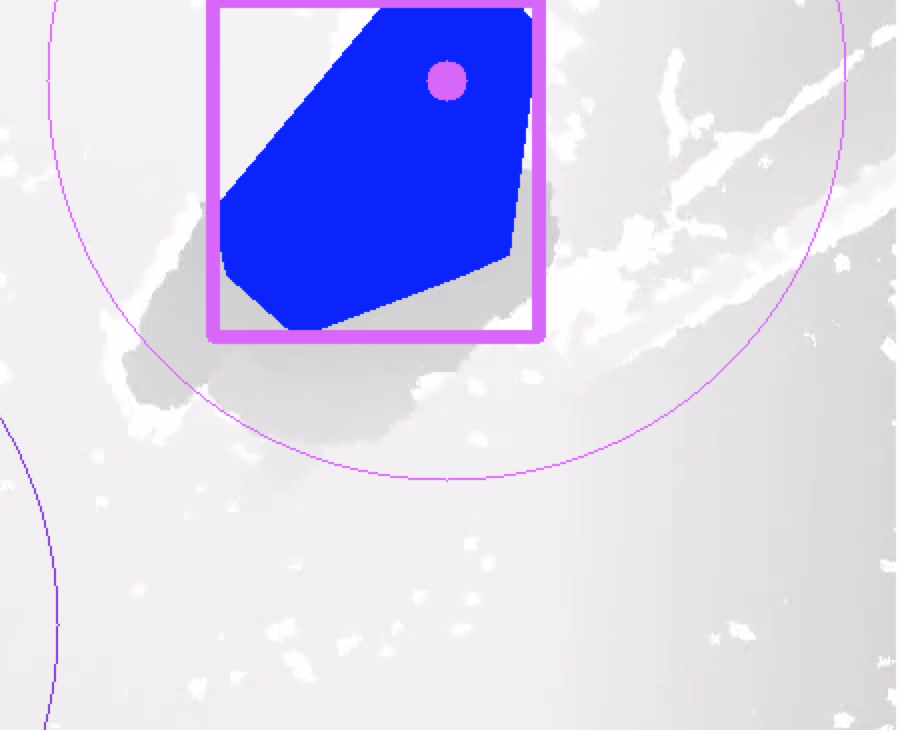
\includegraphics[width=\textwidth]{images/connectMask}
    \caption{Spojená kontúra.}
  \end{minipage}
\end{figure}


Popis algoritmu, pričom všetky kontúry nájdené prostredníctvom funkcie metódy sledovania hraníc, sú uložené v zozname \textit{allCont}:
\begin{enumerate}
  \item Zo zoznamu \textit{allCont} odstránime všetky kontúry, ktoré majú nulový obsah.
  \item Vytvoríme nový zoznam \textit{newContura}, vyberieme prvú kontúru z \textit{allCont}, vložíme do zoznamu \textit{newContura} a označíme ju ako \textit{root}.
  \item V zozname \textit{allCont} nájdeme všetky kontúry vyhovujúce podmienke minimálnej absolútnej vzdialenosti ťažísk kontúr oproti kontúre označenej ako \textit{root}.
  \item Nájdené položky vložíme do zoznamu \textit{newContura}, ostatné označíme ako nový zoznam
  \textit{allCont}.
  \item Pre každú najdenú kontúru označíme ako \textit{root} a  pokračujeme bodom 3.
  \item Všetky kontúry v zozname \textit{newContura} spojíme do jednej kontúry.
  \item Pre každú konturu v zozname \textit{allCont} pokračujeme bodom 2.
  
\end{enumerate}
Inými slovami, algoritmus prechádza všetky kontúry a na základe vzdialenosti ťažiskových bodov ich spája do jedného celku.


Spájanie zoznamu kontúr je realizované prostredníctvom volania funkcie \textit{cv2.convexHull}, ktorá pre množinou bodov, ktoré sú obrysové body oblasti, nájde inú množinu bodov reprezentujúcich jej konvexný obal.

\subsubsection{Filtrácia nevyhovujúcich kontúr}  
Keďže poznáme približnú veľkosť kontúry, ktorej detekcia je cieľom záujmu, všetky ostatné sú nežiaduce a je nutné ich odstrániť. Na základe tejto filtrácie sa program zbaví všetkých náhodných oblastí, ktoré vznikli pôsobením šumu. Túto filtráciu je však možné použiť až po aplikovaní algoritmu pre spájanie kontúr. Je to posledná fáza segmentácie obrazu. 

\subsubsection{Výpočet najvyššieho bodu}
Vďaka tomu, že technológia snímania vytvára hĺbkovú mapu, je možné v rámci každej kontúry definovať lokálne maximum každej oblasti. Pri zvolenej koncepcii snímania, bod patrí do množiny bodov nachádzajúcich sa na vrchnej časti hlavy. Tento bod je významný pri sledovaní pohybu objektu. \vspace{5mm}


Proces nájdenia je definovaný postupom týchto krokov: 
\begin{enumerate}
  \item Vytvoríme prázdnu \textbf{masku} veľkosti snímaného obrazu \textit{np.zeros}.
  \item Do \textbf{masky} vložíme kontúru, ktorej maximálnu oblasť chceme nájsť \textit{cv2.drawContours}.
  \item Nájdeme minimálnu, respektíve maximálnu hodnotu reprezentujúcu najvyšší bod kontúry  \textit{cv2.minMaxLoc(originalFrame, mask=mask)}.
  \item Nájdenú hodnotu použijeme ako prahovú hodnotu a aplikujeme funkciu prahovania s globálnym prahom na originálny obraz. Výsledkom je binárna maska \textit{cv2.threshold}.
  \item Medzi maskou vytvorenou v bode 2 a maskou vytvorenou v bode 4 vykonáme logickú operáciu AND, čoho výsledkom je binárna maska maximálnej oblasti skúmanej kontúry \textit{cv2.bitwise\_and(mask, thresh)}.
  \item Následne môžeme znovu vyhľadať všetky uzavrené oblasti, ktoré vznikli na obraze \textit{cv2.findContours}.
  \item Vyberieme kontúru s najväčším obsahom, pre ktorú vyrátame ťažisko a nájdený bod prehlásime za maximálny bod oblasti.
\end{enumerate}

\subsection{Priradenie kontúr objektom}
V prípade, že sme schopní v každom obraze, ktorý patrí do konštantného toku dát zo snímača vykonať spoľahlivú segmentáciu, je možné postúpiť na objektový level abstrakcie. Objekt je určený sériou rôznych kontúr, medzi ktorými existuje vzájomná závislosť.  

Proces vytvárania a zanikania kontúr aplikácie je založený na dvoch hlavných vlastnostiach:
\begin{itemize}
    \item Pozícia oblasti
    \item Hodnota výškového maxima oblasti
\end{itemize}

Pre každý existujúci objekt na scéne sa vypočíta absolútna vzdialenosť ku všetkým nájdeným oblastiam aktuálneho obrazu. Následne sa vzdialenosti usporiadajú od najmenšej po najväčšiu a odstránia všetky, ktoré sú väčšie ako hraničná hodnota stanovená pri konfigurácii. Priradenia, ktoré ostali v zozname sa aplikujú a aktualizuje sa poloha objektov. V prípade, že kontúre nebol priradený žiadny objekt, vytvorí sa nový a kontúra sa priradí ako inicializačná poloha nového objektu. 

\subsection{Sledovanie objektu}
Pri sledovaní osôb v pohybe dochádza k rôznym problémom, ktorým je nutné venovať veľkú pozornosť. Najčastejšie riešeným problémom je jednoznačne určiť, ktorá \textbf{kontúra bude priradená ktorému objektu}. Vzhľadom na to, že priemerný tok dát z kamier je 15 - 20 snímkov za sekundu, zmeny polohy objektov medzi dvoma za sebou idúcimi snímkami môžu byť natoľko veľké, že sledovanie zlyhá. Druhým vážnym problémom je \textbf{spojenie dvoch kontúr do jednej}, čo spôsobuje vytlačenie jedného z objektov, ktorý stratí kontúru, ktorú by mohol sledovať. Táto situácia môže nastať fyzickým kontaktom dvoch osôb (veľmi blízky prechod, zrazenie sa a iné...). Oba problémy majú spoločné riešenie a tým je predikcia nasledujúcej polohy na základe smeru a rýchlosti, ktorú objekt nadobudol do momentu incidentu.
V rámci implementácie som otestoval dva algoritmy.
\begin{itemize}
    \item Kalmanov filter
    \item Výpočet na základe histórie a rýchlosti
\end{itemize}


\begin{figure}[H]
  \centering
  \begin{minipage}[b]{0.4\textwidth}
    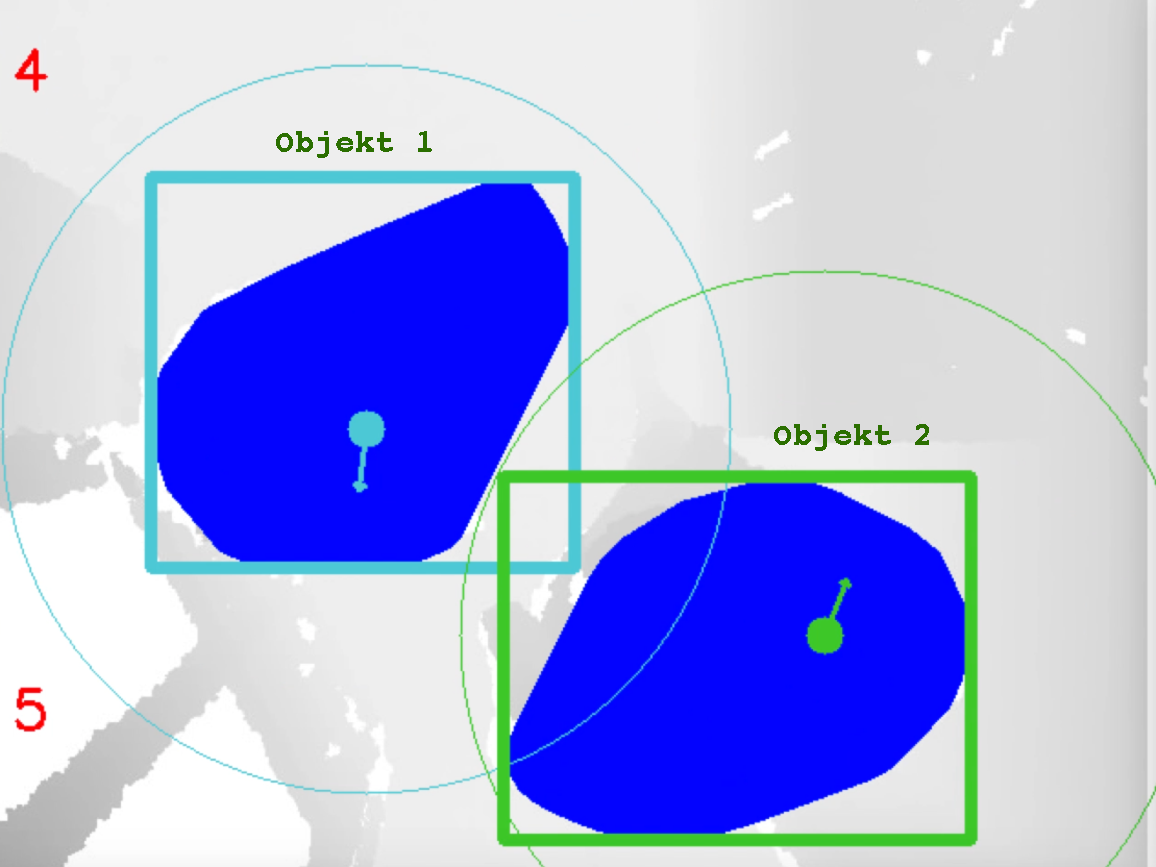
\includegraphics[width=\textwidth]{images/beforeCollision}
    \caption{Moment pred kolíziou dvoch kontúr.}
  \end{minipage}
  \hfill
  \begin{minipage}[b]{0.55\textwidth}
    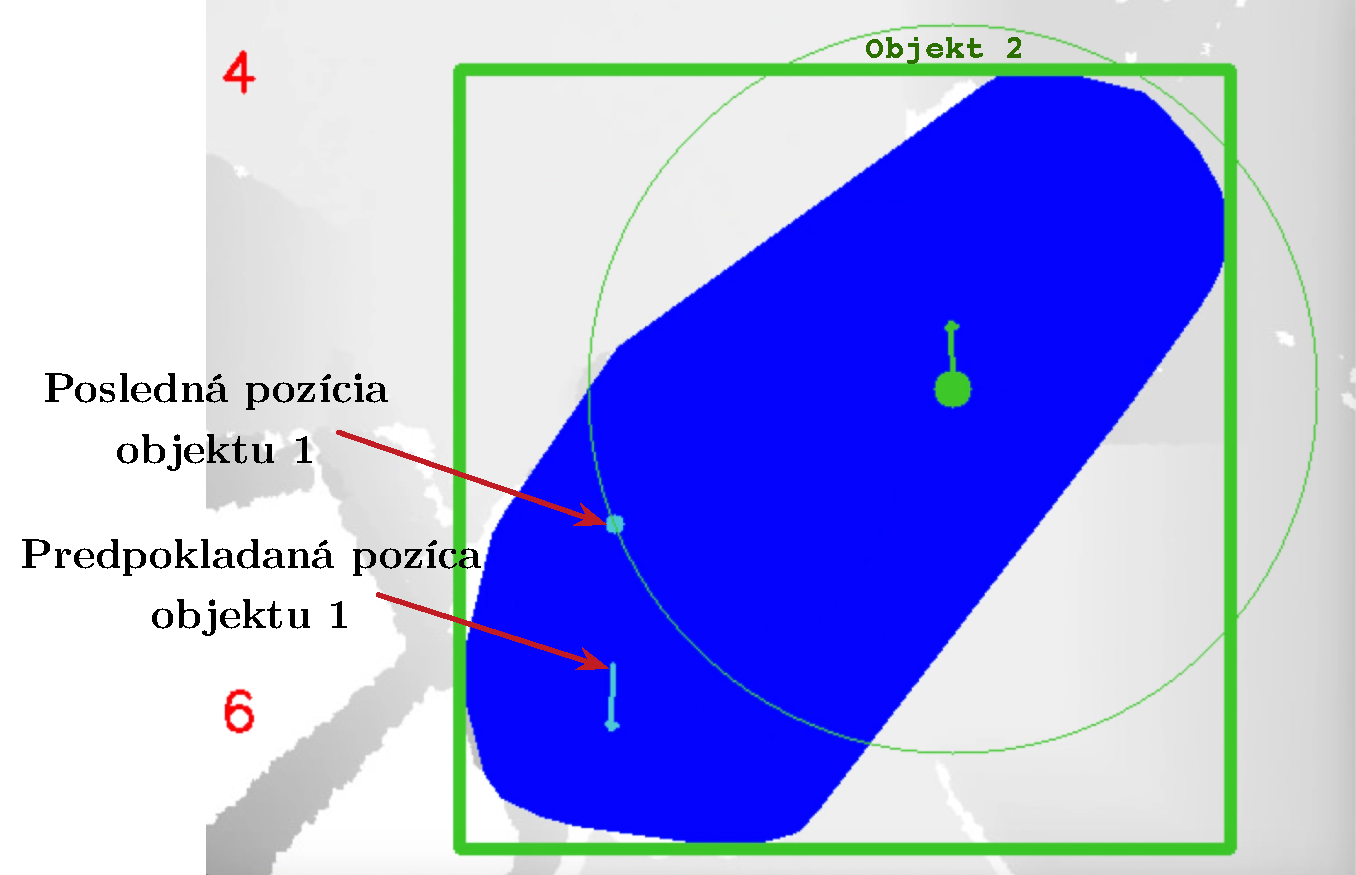
\includegraphics[width=\textwidth]{images/predicate}
    \caption{Využitie predpovedania polohy.}
  \end{minipage}
\end{figure}



\textbf{Kalmanov filter} - Teoretický základ funkčnosti tohto filtra bol opísaný v sekcii \ref{sec:kalman}. Pri implementácii som využil knižnicu \textit{openCV}, ktorá ho obsahuje. Pri testoch som však objavil veľký problém. Kalmanov filter potrebuje pomerne veľkú históriu korekcií na to, aby získal požadovanú presnosť. Priemerný prechod jedného človeka cez virtuálnu bránu, je zachytený na 10 - 20 snímkoch. Podľa testov Kalmanov filter potrebuje na získanie základnej presnosti 5 - 6 korekcií. Tento problém je samozrejme možné riešiť zmenou snímacieho zariadenia alebo umiestnením kamery na vyššie položené miesto, a tým maximalizovať zotrvanie objektov na scéne. 

\textbf{Výpočet na základe histórie a rýchlosti} - Táto metóda je veľmi jednoduchá a opiera sa o vedomosti zo základnej školy. Pre každý objekt vytvoríme históriu, ktorá obsahuje pozíciu a časovú známku. Veľkosť histórie definujeme podľa toho, koľko bodov má ovplyvňovať predikciu nasledujúceho bodu. Proces výpočtu predikcie potom vyzerá tak, že najprv vyrátame moment rýchlosti pre x-ovú aj y-ovú os: 

\begin{figure}[H]
    \centering
    \begin{minipage}[b]{0.45\textwidth}
        \begin{equation}
            v_x = \frac{last_x - first_x} {t}
        \end{equation}
    \end{minipage}
    \hfill
    \begin{minipage}[b]{0.4\textwidth}
        \begin{equation}
            v_y = \frac{last_y - first_y} {t}
        \end{equation}
    \end{minipage}
\end{figure}

kde \textit{last} je najstaršia známa poloha, \textit{first} je najnovšia pozícia a \textit{t} je celkový čas od najstaršieho po najnovší záznam v histórii. Keď máme vypočítané rýchlosti, máme všetko pre určenie predikcie na základe aktuálneho času takto: 

\begin{figure}[H]
    \centering
    \begin{minipage}[b]{0.45\textwidth}
        \begin{equation}
            predicate_x = last_x + v_x * \Delta t
        \end{equation}
    \end{minipage}
    \hfill
    \begin{minipage}[b]{0.4\textwidth}
        \begin{equation}
            predicate_y = last_y + v_y * \Delta t
        \end{equation}
    \end{minipage}
\end{figure}

kde, $\Delta t$ je rozdiel medzi časom hľadanej polohy a časom poslednej známej polohy. Tento výpočet funguje spoľahlivo už pri druhom snímku a pri testoch dosahoval lepšie výsledky ako Kalmanov filter. Z toho dôvodu bol na predikciu polohy využitý práve tento algoritmus. 

\section{Implementácia aplikácie s využitím RGB web kamery}
Implementácia aplikácie s využitím RGB web kamery využíva veľmi podobné stratégie ako aplikácia založená na hĺbkovom snímaní, ktorá bola opísaná vyššie. Dva najvýznamnejšie rozdiely predstavujú:
\begin{itemize}
\item Spôsob vytvárania binárnej masky
\item Určenie významného bodu oblasti - ťažisko oblasti
\end{itemize}

\subsection{Binárna maska}
Princíp snímania webkamery je založený na interakcii CCD čipu  so svetlom prichádzajúcim od pozorovaného objektu. Odrazom svetla od povrchu sa môže odraziť v plnom spektre pod rovnakým uhlom (zrkadlo, lesklé objekty), alebo svetlo prenikne do objektu, kde sa časť vlnovej dĺžky sa pohltí a zvyšok sa odrazí. Senzor teda vníma spektrum odrazeného svetla ako určitú farbu.

Ak by sme aj v tomto prípade chceli využiť \textbf{metódu prahovania}, museli by sme zabezpečiť, aby priestor snímaný kamerou bol vždy farebne iný od objektov prechádzajúcich skrz. Tak by bolo možné odfiltrovať všetky pixle s vlnovou dĺžkou odrazeného svetla (farbou) zodpovedajúcou pozadiu. Ďalej by bolo nutné zabezpečiť homogénne osvetlenie scény, aby bol zabezpečený dostatok svetla. Vzhľadom na všetky tieto problémy je metóda nepoužiteľná pre daný účel.

Výhodnejšou stratégiou predstavuje použitie \textbf{metódy odčítavania pozadia} (\textit{Background Subtractor}). Je to analytická metóda, pre postupné učenie sa pozadia a jeho odčítavanie od obrazu v popredí. Výsledkom je binárna maska obrazu, kde pixel, ktorý sa zmenil má logickú hodnotu 1 a pixel, ktorý je pozadím 0. 

\subsubsection{Požiadavky na výkon}
Algoritmy pre odčítavanie pozadia sú veľmi náročné na výpočtový výkon a to priamoúmerné rozlíšeniu spracovávaného obrazu. V rámci implementácie boli testované MOG\footnote{Odkaz na publikáciu: \url{http://link.springer.com/chapter/10.1007\%2F978-1-4615-0913-4_11}}, MOG2\footnote{Odkaz na publikáciu: \url{http://ieeexplore.ieee.org/document/1333992/}}, KNN.

Najlepší pomer kvality binárnej masky a výkonu potrebného na jej získanie má \textit{KNN (K-nearest)}. Jeho implementáciu obsahuje knižnica  \textit{cv2.createBackgroundSubtractorKNN()}. Je veľmi efektívny, ak sa v popredí obrazu mení len jeho malá časť. 

\subsubsection{Paralelné spracovávanie}
Pri implementácii ďalších testoch sa však ukázalo, že pri spustení aplikácie na Rasperry PI rýchlosť spracovávania jednotlivých obrazov bola nedostatočná (8-10 FPS). Pre zvýšenie priepustnosti spracovávania bolo nutné zlepšiť vyťaženie viacerých jadier procesora súčasne (asynchrónny prístup). 

Implementácia asynchrónneho spracovania funguje na princípe generácie množstva vlákien, ktoré sú spolu synchronizované na základe zámkov. V prvom kroku algoritmu sa inicializuje \textit{videostream} a \textit{background substractor}. Následne sa vygeneruje N vlákien (\textit{workers}). Každé vlákno obsahuje jeden zámok na čítanie ďalšieho snímku obrazu a druhý zámok pre zápis do zoznamu spracovaných snímkov. Tie sa pri vytváraní uzamknú. Každé vlákno v nekonečnom cykle vykonáva:
\begin{enumerate}
\item Uzamknutie zámku pre čítanie ďalšieho snímku
\item Čítanie ďalšieho snímku 
\item Otvorenie zámku pre čítanie nasledujúceho vlákna \textit{(i + 1)}
\item Zahájenie výpočtu Bacground substractoru
\item Uzamknutie zámku pre zápis výsledku do zoznamu výsledkov
\item Vloženie výsledku operácie do zoznamu výsledkov 
\item Otvorenie zámku pre vloženie výsledku ďalšieho vlákna \textit{(i + 1)} 
\end{enumerate}

Algoritmus bol testovaný na \textit{Raspberry PI 3}. Nasledujúce grafy prezentujú závislosť rýchlosti spracovávania snímkov na veľkosti snímaného obrazu a počte vlákien algoritmu:

\begin{figure}[H]
  \centering
  \begin{minipage}[b]{0.49\textwidth}
    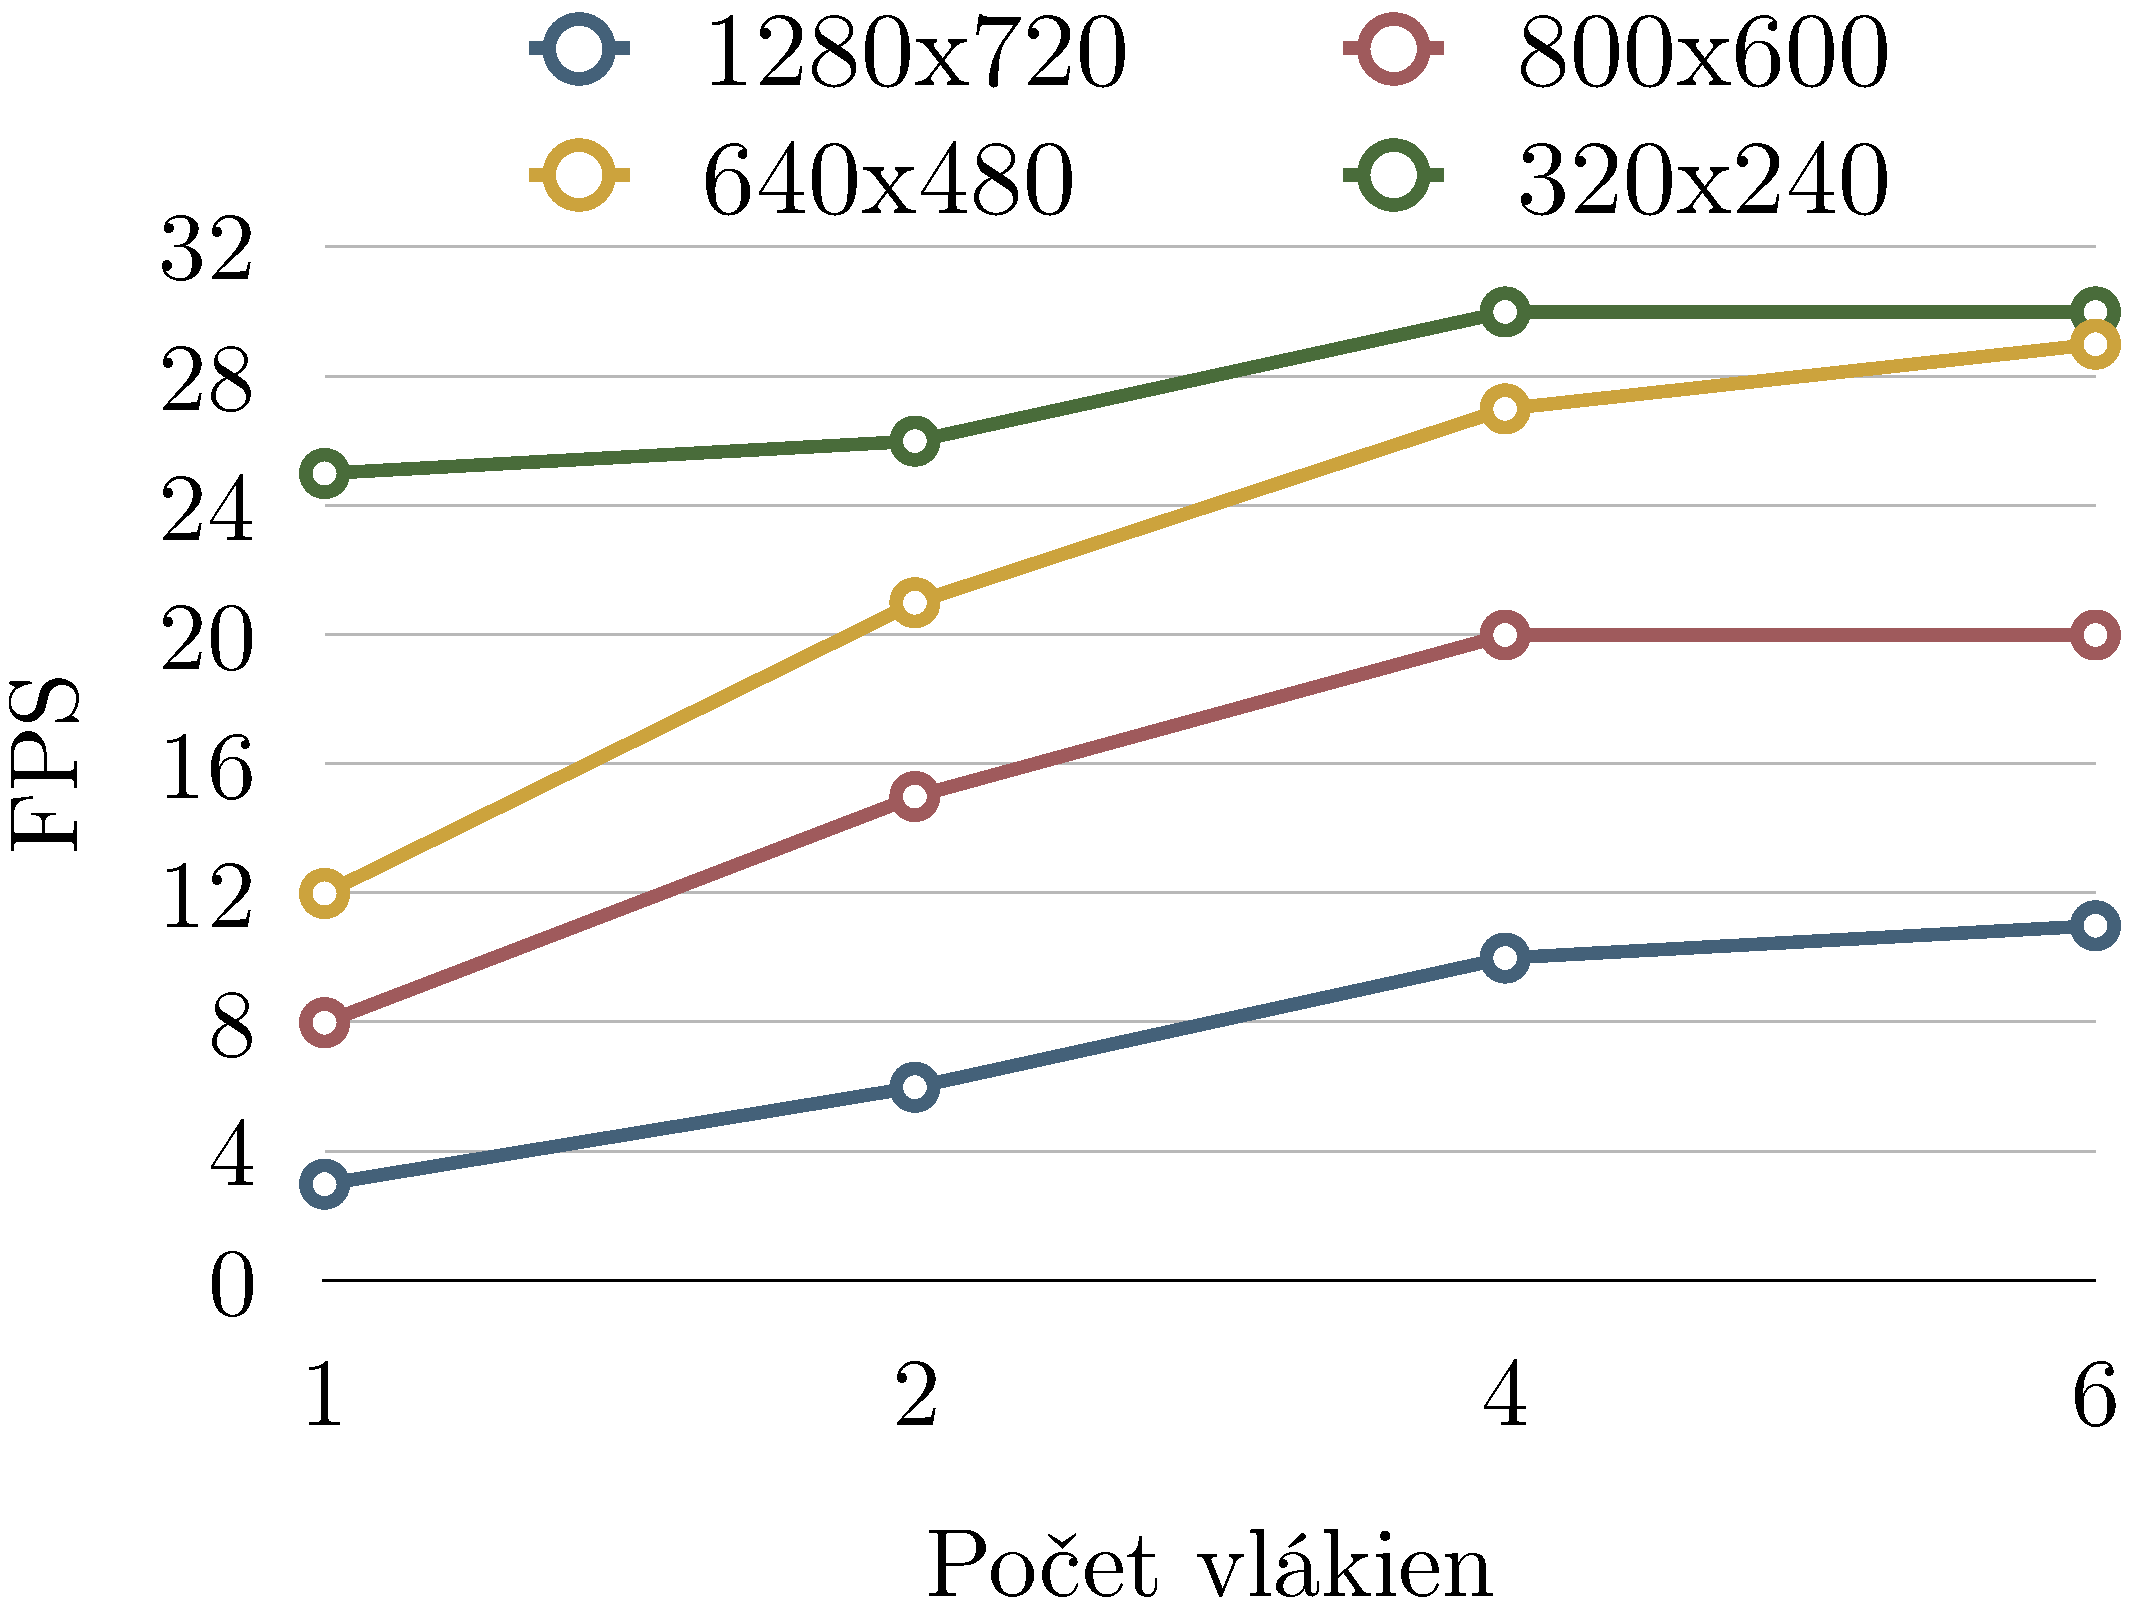
\includegraphics[width=\textwidth]{images/substractorCalm}
    \caption{Nemenná scéna.}
  \end{minipage}
  \hfill
  \begin{minipage}[b]{0.49\textwidth}
    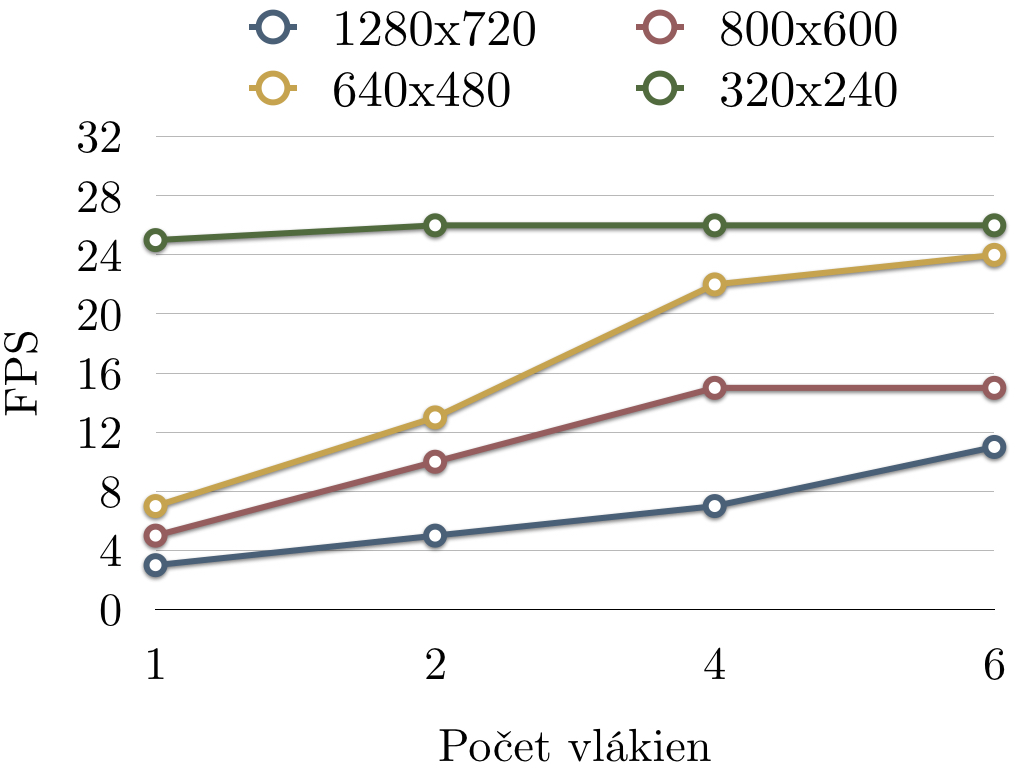
\includegraphics[width=\textwidth]{images/substractorNormal}
    \caption{Priemerne veľký pohyb na scéne.}
  \end{minipage}
\end{figure}

Z testov vyplýva, že algoritmus najlepšie pracuje pri snímacom rozlíšení \textbf{640*480 pixlov} s využitím \textbf{štyroch asynchrónnych vlákien}. Pri týchto atribútoch dosiahnutá hodnota snímkov za sekundu (FPS) aj veľkosť rozlíšenia dostatočná pre ďalšie spracovanie. 




  \chapter{Výsledky práce a možnosti rozšírenia}
  
\chapter{Záver}
Cieľom tejto práce bolo vytvoriť aplikáciu, ktorá bude schopná počítať prechody osôb s čo najväčšou presnosťou a zachová si  priaznivú cenu. V rámci práce boli vytvorené dve aplikácie. Jedna pre snímanie priestoru virtuálnej brány za pomoci 2D technológie a druhá, ktorá používa pre snímanie aktívne hĺbkomery (príloha \ref{pr:CD}).

V prípade aplikácie využívajúcej 2D snímanie sa podarilo vytvoriť nasaditeľnú aplikáciu, ktorej úspešnosť detekcie sa pohybuje medzi \textbf{90 - 94\%}. Cenu takéhoto zariadenia sa podarilo stlačiť na \textbf{70 EUR} vďaka použitiu malého a lacného počítača Rraspberry Pi a štandardnej širokouhlej webkamery. Nízka cena zariadenia dovoľuje použiť takýto produkt pre rôzne maloobchodné prevádzky, ktoré potrebujú informácie o počte návštev zo štatistických dôvodov a nižšia spoľahlivosť zariadenia im neprekáža. Takéto zariadenia majú potenciál nahradiť nepresné IR závory, ktoré sú stále veľmi často používané kvôli cenovej nedostupnosti presnejších riešení.

V prípade druhej aplikácie, ktorá detekuje prechod osôb za pomocí hĺbkového snímku priestoru brány, bolo na začiatok nutné vybrať najvhodnejší hĺbkomer. V rámci práce boli k dispozícii žiaľ len tri a všetky používali technológiu aktívnej triangulácie (sekcia~\ref{sec:activeDeep}). Napriek tomu sa podarilo vytvoriť systém pre porovnanie kvality hĺbkového snímku na základe priemerného počtu chybne nameraných pixlov. Práca ukázala, že Kinect 360 má väčšiu odolnosť voči interferencii denného svetla avšak nie je možné určiť, ktorý hĺbkový snímač je pre aplikáciu najlepší. Je to z dôvodu rozdielnych zorných polí kamier. Preto na výber najvhodnejšej kamery je nutné poznať presné miesto nasadenia systému. Nameraná úspešnosť aplikácie vytvorenej v rámci tejto práce bola \textbf{96 - 98\%}. Cena sa pohybuje okolo \textbf{150 - 220 EUR} v závislosti na type použitého hĺbkomera, keďže predstavuje najdrahšiu položku celého produktu. Vďaka vysokej presnosti je tento typ aplikácie vhodný na príklad v aplikáciach objektovej bezpečnosti v spojení s ďalším systémom overujúcim identitu prechádzaného objektu alebo v aplikáciach, kde je potrebné zaznámenávať väčšie množstvo informácií, ako napríklad výšku človeka.


  % Pouzita literatura / Bibliography
  % ----------------------------------------------
\ifslovak
  \makeatletter
  \def\@openbib@code{\addcontentsline{toc}{chapter}{Literatúra}}
  \makeatother
  \bibliographystyle{bib-styles/czechiso}
\else
  \ifczech
    \makeatletter
    \def\@openbib@code{\addcontentsline{toc}{chapter}{Literatura}}
    \makeatother
    \bibliographystyle{bib-styles/czechiso}
  \else 
    \makeatletter
    \def\@openbib@code{\addcontentsline{toc}{chapter}{Bibliography}}
    \makeatother
    \bibliographystyle{bib-styles/englishiso}
    \bibliographystyle{alpha}
  \fi
\fi
  \begin{flushleft}
  \bibliography{projekt-20-literatura-bibliography}
  \end{flushleft}

  % vynechani stranky v oboustrannem rezimu
  % Skip the page in the two-sided mode
  \iftwoside
    \cleardoublepage
  \fi

  % Prilohy / Appendices
  % ---------------------------------------------
  \appendix
\ifczech
  \renewcommand{\appendixpagename}{Přílohy}
  \renewcommand{\appendixtocname}{Přílohy}
  \renewcommand{\appendixname}{Příloha}
\fi
\ifslovak
  \renewcommand{\appendixpagename}{Prílohy}
  \renewcommand{\appendixtocname}{Prílohy}
  \renewcommand{\appendixname}{Príloha}
\fi
  \appendixpage

% vynechani stranky v oboustrannem rezimu
% Skip the page in the two-sided mode
\iftwoside
  \cleardoublepage
\fi
  
\ifslovak
%  \section*{Zoznam príloh}
%  \addcontentsline{toc}{section}{Zoznam príloh}
\else
  \ifczech
%    \section*{Seznam příloh}
%    \addcontentsline{toc}{section}{Seznam příloh}
  \else
%    \section*{List of Appendices}
%    \addcontentsline{toc}{section}{List of Appendices}
  \fi
\fi
  \startcontents[chapters]
  % seznam příloh / list of appendices
  % \printcontents[chapters]{l}{0}{\setcounter{tocdepth}{2}}
  
  % vynechani stranky v oboustrannem rezimu
  \iftwoside
    \cleardoublepage
  \fi
  
\chapter{Program pre čítanie kamery Orbbec Astra S}
\label{pr:astra}
\begin{lstlisting}[language=Python]
import cv2
import numpy as np
from primesense import openni2
from primesense import _openni2 as c_api
def initCapture():
    openni2.initialize("./lib/openni2") #Path to libOpenNI2.dylib
    dev = openni2.Device.open_any()
    depth_stream = dev.create_depth_stream()
    depth_stream.start()
    depth_stream.set_video_mode(c_api.OniVideoMode(pixelFormat = 
            c_api.OniPixelFormat.ONI_PIXEL_FORMAT_DEPTH_100_UM,
        resolutionX = 640, resolutionY = 480, fps = 30))
    return depth_stream

def cap_read(depth_stream):
    raw_frame = depth_stream.read_frame()
    frame_data = raw_frame.get_buffer_as_uint16()
    img = np.frombuffer(frame_data, dtype=np.uint16)
    img.shape = (1, 480, 640)
    img = np.concatenate((img, img, img), axis=0)
    img = np.swapaxes(img, 0, 2)
    img = np.swapaxes(img, 0, 1)
    img8 = (img/256).astype('uint8')
    img8 = (255-img8)
    return img8
depth_stream = initCapture()
while True:
    frame = cap_read(depth_stream)
    grayFrame = cv2.cvtColor(frame, cv2.COLOR_BGR2GRAY)
    cv2.imshow("image", frame)
    cv2.waitKey(1)
openni2.unload()

\end{lstlisting}

\chapter{Program pre nahrávanie kamery Intel RealSence SR30}
\label{pr:realSence}
\begin{lstlisting}[language=Python]
import time
import numpy as np
import cv2
import pyrealsense as pyrs
import sys

def cap_read(dev):
    dev.wait_for_frame()
    d = dev.depth * dev.depth_scale * 255
    d = d.astype('uint8')
    d = (255-d)
    return d

record = False
if "-r" in sys.argv:
    record = True
    fourcc = cv2.VideoWriter_fourcc(*'XVID')
    out = cv2.VideoWriter('intelRealSenceSR300.avi',
          fourcc, 30.0, (640,480))

pyrs.start()
dev = pyrs.Device()

while True:
    frame = cap_read(dev)
    frame = cv2.cvtColor(frame, cv2.COLOR_GRAY2BGR)
    if record:
        out.write(frame)

    cv2.imshow('frame', frame)
    if cv2.waitKey(1) & 0xFF == ord('q'):
        break
\end{lstlisting}


\chapter{Program pre nahrávanie kamery Kinect 360}
\label{pr:kinect}
\begin{lstlisting}[language=Python]
import numpy as np
import cv2
import freenect

def getDepthMap():    
    depth, timestamp = freenect.sync_get_depth()
    np.clip(depth, 0, 2**10 - 1, depth)
    depth >>= 2
    depth = depth.astype(np.uint8)
    return depth

fourcc = cv2.VideoWriter_fourcc(*'XVID')
record_cap = cv2.VideoWriter('output.avi',fourcc, 20.0, (640,480))
while(True):
	depth = getDepthMap()
	frame = cv2.cvtColor(depth,cv2.COLOR_GRAY2BGR)
	record_cap.write(frame)
	cv2.imshow('frame',frame)
	if cv2.waitKey(1) & 0xFF == ord('q'):
	    break
\end{lstlisting}


\chapter{Program pre výpočet metriky hĺbkovej kamery}
\label{pr:metric}
\begin{lstlisting}[language=Python]
import numpy as np
import cv2
import sys

cap = cv2.VideoCapture("./4/orbbecAstraS.mov")
limint = 1000
count = 0
sumPixels = 0 
while(True):
    # Capture frame-by-frame
    ret, frame = cap.read()

    if count == limint:
        print "Resolution: ", len(frame), "x", len(frame[0]) 
        print "AVG pixels for frame: ", sumPixels / count
        sys.exit(0)

    frame = frame[:,40:]
    sumPixels += np.count_nonzero(frame == 255)
    count += 1
    cv2.imshow('fgrayrame',frame)
    if cv2.waitKey(1) & 0xFF == ord('q'):
        break

# When everything done, release the capture
cap.release()
cv2.destroyAllWindows()
\end{lstlisting}

\chapter{Obsah DVD}
\label{pr:CD}
DVD nosič obsahuje: 
\begin{itemize}
    \item Zdrojové kódy aplikácie založenej na snímaní 2D
    \item Zdrojové kódy aplikácie založenej na snímaní 3D
    \item Vzorka testovacích dát 
    \item Kompletný obraz pamäťovej karty Rraspberry Pi
    \item Demo aplikáce hranového detektora, globálneho prahovania, metód lokálneho prahovania využitých v práci
    
\end{itemize}
\label{pr:metric} % viz. prilohy.tex / see prilohy.tex
\end{document}
